\documentclass[twoside]{book}

% Packages required by doxygen
\usepackage{fixltx2e}
\usepackage{calc}
\usepackage{doxygen}
\usepackage[export]{adjustbox} % also loads graphicx
\usepackage{graphicx}
\usepackage[utf8]{inputenc}
\usepackage{makeidx}
\usepackage{multicol}
\usepackage{multirow}
\PassOptionsToPackage{warn}{textcomp}
\usepackage{textcomp}
\usepackage[nointegrals]{wasysym}
\usepackage[table]{xcolor}

% Font selection
\usepackage[T1]{fontenc}
\usepackage[scaled=.90]{helvet}
\usepackage{courier}
\usepackage{amssymb}
\usepackage{sectsty}
\renewcommand{\familydefault}{\sfdefault}
\allsectionsfont{%
  \fontseries{bc}\selectfont%
  \color{darkgray}%
}
\renewcommand{\DoxyLabelFont}{%
  \fontseries{bc}\selectfont%
  \color{darkgray}%
}
\newcommand{\+}{\discretionary{\mbox{\scriptsize$\hookleftarrow$}}{}{}}

% Page & text layout
\usepackage{geometry}
\geometry{%
  a4paper,%
  top=2.5cm,%
  bottom=2.5cm,%
  left=2.5cm,%
  right=2.5cm%
}
\tolerance=750
\hfuzz=15pt
\hbadness=750
\setlength{\emergencystretch}{15pt}
\setlength{\parindent}{0cm}
\setlength{\parskip}{3ex plus 2ex minus 2ex}
\makeatletter
\renewcommand{\paragraph}{%
  \@startsection{paragraph}{4}{0ex}{-1.0ex}{1.0ex}{%
    \normalfont\normalsize\bfseries\SS@parafont%
  }%
}
\renewcommand{\subparagraph}{%
  \@startsection{subparagraph}{5}{0ex}{-1.0ex}{1.0ex}{%
    \normalfont\normalsize\bfseries\SS@subparafont%
  }%
}
\makeatother

% Headers & footers
\usepackage{fancyhdr}
\pagestyle{fancyplain}
\fancyhead[LE]{\fancyplain{}{\bfseries\thepage}}
\fancyhead[CE]{\fancyplain{}{}}
\fancyhead[RE]{\fancyplain{}{\bfseries\leftmark}}
\fancyhead[LO]{\fancyplain{}{\bfseries\rightmark}}
\fancyhead[CO]{\fancyplain{}{}}
\fancyhead[RO]{\fancyplain{}{\bfseries\thepage}}
\fancyfoot[LE]{\fancyplain{}{}}
\fancyfoot[CE]{\fancyplain{}{}}
\fancyfoot[RE]{\fancyplain{}{\bfseries\scriptsize Generated by Doxygen }}
\fancyfoot[LO]{\fancyplain{}{\bfseries\scriptsize Generated by Doxygen }}
\fancyfoot[CO]{\fancyplain{}{}}
\fancyfoot[RO]{\fancyplain{}{}}
\renewcommand{\footrulewidth}{0.4pt}
\renewcommand{\chaptermark}[1]{%
  \markboth{#1}{}%
}
\renewcommand{\sectionmark}[1]{%
  \markright{\thesection\ #1}%
}

% Indices & bibliography
\usepackage{natbib}
\usepackage[titles]{tocloft}
\setcounter{tocdepth}{3}
\setcounter{secnumdepth}{5}
\makeindex

% Hyperlinks (required, but should be loaded last)
\usepackage{ifpdf}
\ifpdf
  \usepackage[pdftex,pagebackref=true]{hyperref}
\else
  \usepackage[ps2pdf,pagebackref=true]{hyperref}
\fi
\hypersetup{%
  colorlinks=true,%
  linkcolor=blue,%
  citecolor=blue,%
  unicode%
}

% Custom commands
\newcommand{\clearemptydoublepage}{%
  \newpage{\pagestyle{empty}\cleardoublepage}%
}

\usepackage{caption}
\captionsetup{labelsep=space,justification=centering,font={bf},singlelinecheck=off,skip=4pt,position=top}

%===== C O N T E N T S =====

\begin{document}

% Titlepage & ToC
\hypersetup{pageanchor=false,
             bookmarksnumbered=true,
             pdfencoding=unicode
            }
\pagenumbering{roman}
\begin{titlepage}
\vspace*{7cm}
\begin{center}%
{\Large Decomposer \\[1ex]\large 0.\+9 }\\
\vspace*{1cm}
{\large Generated by Doxygen 1.8.11}\\
\end{center}
\end{titlepage}
\clearemptydoublepage
\tableofcontents
\clearemptydoublepage
\pagenumbering{arabic}
\hypersetup{pageanchor=true}

%--- Begin generated contents ---
\chapter{Decomposer}
\label{index}\hypertarget{index}{}Decomposer is a relational decomposition tool that uses the functional dependencies of the relation to identify normal form and generate the sub-\/relations.

It uses the either one of two algorithms -\/ Functional Dependencies Preserving Lossless decomposition or the Non Functional Dependencies Preserving Lossless decomposition. The FD Preserving algorithm guarantees that the sub-\/relations are at least in third normal form and all the original F\+Ds are preserved. The non FD preserving may not preserve all the original F\+Ds but it guarantees that all the sub-\/relations are in BC Normal Form.

This is a command line tool built by using G\+CC the G\+NU compiler collection on Linux platform. Using command line interface, the user can provide the information about the functional dependencies and the attributes of the relations. The user then can perform decomposition of the relation or find out about analysis of the relation.

The \textquotesingle{}relation\textquotesingle{} in this tool represents the entity which have the identifying name, a set of attributes and a set of functional dependencies among these attributes. The \textquotesingle{}attribute\textquotesingle{} represents characteristics of the relational entity. The dependencies defines the deterministic relation between set of attributes.

For example, R(a,b,c,d,e) \{a-\/$>$b , ab-\/$>$de\} In above example the relation name is R, the set of attributes is \{a,b,c,d,e\} and functional dependencies are \{a\} -\/$>$ \{b\} and \{a,b\} -\/$>$ \{d,e\}

Along with decomposition the user can choose different operation to be performed on the relation which includes finding minimal cover for dependency set, finding the candidate key for the relation, testing normal form of the relation and getting the dependencies that violates the particular normal form.

A command line based interactive menu driven user interface will be used by the application to accept user input and perform corresponding action. The Makefile can be use to compile the source code create the executable. make run command can be use to compile and run the executable.

The testing for application is performed by using the cppunit library. The unit tests are performed on various class methods and global functions.

The application can be started by using make run command or the executable program Decomposer can be used to start the application. The \hyperlink{class_relation}{Relation} object will be initialized first by providing details about relation name, attribute set and dependency set. The user can modify or reinitialize the the \hyperlink{class_relation}{Relation} object as required. The user can selects the different operation to be performed on this object using menu choice. Note\+: It is assumed that the input relation object is in at least first normal form, meaning the application currently do not supports the multivalued attributes.

\begin{DoxyAuthor}{Author}
Ashish D. Kharde 
\end{DoxyAuthor}

\chapter{Hierarchical Index}
\section{Class Hierarchy}
This inheritance list is sorted roughly, but not completely, alphabetically\+:\begin{DoxyCompactList}
\item \contentsline{section}{Dependency}{\pageref{class_dependency}}{}
\item \contentsline{section}{Relation}{\pageref{class_relation}}{}
\item \contentsline{section}{setstr\+\_\+compare}{\pageref{classsetstr__compare}}{}
\item unary\+\_\+function\begin{DoxyCompactList}
\item \contentsline{section}{Violation}{\pageref{struct_violation}}{}
\end{DoxyCompactList}
\item \contentsline{section}{User\+Interface}{\pageref{class_user_interface}}{}
\end{DoxyCompactList}

\chapter{Class Index}
\section{Class List}
Here are the classes, structs, unions and interfaces with brief descriptions\+:\begin{DoxyCompactList}
\item\contentsline{section}{\hyperlink{class_dependency}{Dependency} \\*That represents the functional dependency of the relation using the attribute set }{\pageref{class_dependency}}{}
\item\contentsline{section}{\hyperlink{class_relation}{Relation} \\*That represents the relation entity }{\pageref{class_relation}}{}
\item\contentsline{section}{\hyperlink{classsetstr__compare}{setstr\+\_\+compare} \\*The function object class for less-\/than inequality comparison of the set of string }{\pageref{classsetstr__compare}}{}
\item\contentsline{section}{\hyperlink{class_user_interface}{User\+Interface} \\*That represents the interface class which interacts with the user using command line interface and performs the actions accordingly }{\pageref{class_user_interface}}{}
\item\contentsline{section}{\hyperlink{struct_violation}{Violation} \\*A unary functor class used to test the dependency for the normal form violation }{\pageref{struct_violation}}{}
\end{DoxyCompactList}

\chapter{File Index}
\section{File List}
Here is a list of all documented files with brief descriptions\+:\begin{DoxyCompactList}
\item\contentsline{section}{\hyperlink{declaration_8h}{declaration.\+h} \\*Includes declaration of classes and definition of comparator class }{\pageref{declaration_8h}}{}
\item\contentsline{section}{\hyperlink{dependency_8cc}{dependency.\+cc} \\*Includes definitions of the \hyperlink{class_dependency}{Dependency} class members defined in the \hyperlink{dependency_8h}{dependency.\+h} file }{\pageref{dependency_8cc}}{}
\item\contentsline{section}{\hyperlink{dependency_8h}{dependency.\+h} \\*Includes declaration for the class \hyperlink{class_dependency}{Dependency} and its members }{\pageref{dependency_8h}}{}
\item\contentsline{section}{\hyperlink{relation_8cc}{relation.\+cc} \\*Includes definitions of the \hyperlink{class_relation}{Relation} class members defined in the \hyperlink{relation_8h}{relation.\+h} file }{\pageref{relation_8cc}}{}
\item\contentsline{section}{\hyperlink{relation_8h}{relation.\+h} \\*Includes declaration for the class \hyperlink{class_relation}{Relation} and its members }{\pageref{relation_8h}}{}
\item\contentsline{section}{\hyperlink{template__def_8h}{template\+\_\+def.\+h} \\*Contains the definition for various utility template functions }{\pageref{template__def_8h}}{}
\item\contentsline{section}{\hyperlink{typedef_8h}{typedef.\+h} \\*Defines the global type alias for data-\/types }{\pageref{typedef_8h}}{}
\item\contentsline{section}{\hyperlink{user__interface_8cc}{user\+\_\+interface.\+cc} \\*Includes definitions of the \hyperlink{class_user_interface}{User\+Interface} class members defined in the \hyperlink{user__interface_8h}{user\+\_\+interface.\+h} file }{\pageref{user__interface_8cc}}{}
\item\contentsline{section}{\hyperlink{user__interface_8h}{user\+\_\+interface.\+h} \\*Includes declaration for the class \hyperlink{class_user_interface}{User\+Interface} and its members }{\pageref{user__interface_8h}}{}
\item\contentsline{section}{\hyperlink{utility_8cc}{utility.\+cc} \\*Specifies the definitions for the global non-\/member functions defined in \hyperlink{utility_8h}{utility.\+h} header file }{\pageref{utility_8cc}}{}
\item\contentsline{section}{\hyperlink{utility_8h}{utility.\+h} \\*Defines the prototypes for the global non-\/member functions }{\pageref{utility_8h}}{}
\item\contentsline{section}{\hyperlink{violation_8h}{violation.\+h} \\*Includes declaration of functor class \hyperlink{struct_violation}{Violation} used to check violation of any normal form by the \hyperlink{class_dependency}{Dependency} for a \hyperlink{class_relation}{Relation} object }{\pageref{violation_8h}}{}
\end{DoxyCompactList}

\chapter{Class Documentation}
\hypertarget{class_dependency}{}\section{Dependency Class Reference}
\label{class_dependency}\index{Dependency@{Dependency}}


The \hyperlink{class_dependency}{Dependency} class that represents the functional dependency of the relation using the attribute set.  




{\ttfamily \#include $<$dependency.\+h$>$}

\subsection*{Public Member Functions}
\begin{DoxyCompactItemize}
\item 
\hyperlink{class_dependency_a11db83a63b7dbff6878e621c3ea05303}{$\sim$\+Dependency} ()
\item 
\hyperlink{class_dependency_a626387359a1896a2e39fe27884ed4ce5}{Dependency} (const \hyperlink{class_dependency}{Dependency} \&orig)
\item 
bool \hyperlink{class_dependency_a78821e0db3f417a24b728d38e7d8ff47}{operator$<$} (const \hyperlink{class_dependency}{Dependency} \&) const 
\item 
\hyperlink{typedef_8h_aa234bdb39b1698c1d4955072cfb3195f}{set\+\_\+str} \hyperlink{class_dependency_a75b5b75d47219e1731105d865abcedcf}{get\+Lhs} () const 
\item 
\hyperlink{typedef_8h_aa234bdb39b1698c1d4955072cfb3195f}{set\+\_\+str} \hyperlink{class_dependency_ae14affe4b2559610e997a507d9f331dc}{get\+Rhs} () const 
\item 
\hyperlink{typedef_8h_aa234bdb39b1698c1d4955072cfb3195f}{set\+\_\+str} \hyperlink{class_dependency_aa6638880326df07b4715028f6e8e1eff}{get\+Attribs} () const 
\end{DoxyCompactItemize}
\subsection*{Friends}
\begin{DoxyCompactItemize}
\item 
class {\bfseries Relation}\hypertarget{class_dependency_a7ee004262f27f8c916688911a71e3aa1}{}\label{class_dependency_a7ee004262f27f8c916688911a71e3aa1}

\item 
class {\bfseries dependency\+\_\+test}\hypertarget{class_dependency_a7f472ce92e998f92bf7b3858a37c9840}{}\label{class_dependency_a7f472ce92e998f92bf7b3858a37c9840}

\item 
class {\bfseries relation\+\_\+test}\hypertarget{class_dependency_a63c24e6ee30b65a5c236cef9ff6669bf}{}\label{class_dependency_a63c24e6ee30b65a5c236cef9ff6669bf}

\item 
ostream \& \hyperlink{class_dependency_a9fb9b97e81034d3b367ad1efc7bb6347}{operator$<$$<$} (ostream \&, const \hyperlink{class_dependency}{Dependency} \&)\hypertarget{class_dependency_a9fb9b97e81034d3b367ad1efc7bb6347}{}\label{class_dependency_a9fb9b97e81034d3b367ad1efc7bb6347}

\begin{DoxyCompactList}\small\item\em Insert \hyperlink{class_dependency}{Dependency} object into stream. \end{DoxyCompactList}\end{DoxyCompactItemize}


\subsection{Detailed Description}
The \hyperlink{class_dependency}{Dependency} class that represents the functional dependency of the relation using the attribute set. 

The \hyperlink{class_dependency}{Dependency} class contains the data member that represents the left-\/hand side and right-\/hand of the functional dependency. Both lhs and rhs are considered as the set of attributes. Attributes will be represented by the string representing its name. Note that this class have private constructor which restricts the creation of its object other than its friend member functions and class. The object of this class can be constructed in the \hyperlink{class_relation}{Relation} class methods. This is to ensure the fact that dependency belongs to a particular relation and to identify that unique relation. 

\subsection{Constructor \& Destructor Documentation}
\index{Dependency@{Dependency}!````~Dependency@{$\sim$\+Dependency}}
\index{````~Dependency@{$\sim$\+Dependency}!Dependency@{Dependency}}
\subsubsection[{\texorpdfstring{$\sim$\+Dependency()}{~Dependency()}}]{\setlength{\rightskip}{0pt plus 5cm}Dependency\+::$\sim$\+Dependency (
\begin{DoxyParamCaption}
{}
\end{DoxyParamCaption}
)}\hypertarget{class_dependency_a11db83a63b7dbff6878e621c3ea05303}{}\label{class_dependency_a11db83a63b7dbff6878e621c3ea05303}
Destructor of the \hyperlink{class_dependency}{Dependency} class.

The destructor clears the string objects from the both lhs and rhs data member attributes sets. \index{Dependency@{Dependency}!Dependency@{Dependency}}
\index{Dependency@{Dependency}!Dependency@{Dependency}}
\subsubsection[{\texorpdfstring{Dependency(const Dependency \&orig)}{Dependency(const Dependency &orig)}}]{\setlength{\rightskip}{0pt plus 5cm}Dependency\+::\+Dependency (
\begin{DoxyParamCaption}
\item[{const {\bf Dependency} \&}]{orig}
\end{DoxyParamCaption}
)}\hypertarget{class_dependency_a626387359a1896a2e39fe27884ed4ce5}{}\label{class_dependency_a626387359a1896a2e39fe27884ed4ce5}
The copy constructor of the \hyperlink{class_dependency}{Dependency} class.


\begin{DoxyParams}{Parameters}
{\em orig} & is the \hyperlink{class_dependency}{Dependency} object which to be copied to the newly constructed object\\
\hline
\end{DoxyParams}
The copy constructor initializes the lhs and rhs data members of the class from the corresponding data members of the parameter object. 

\subsection{Member Function Documentation}
\index{Dependency@{Dependency}!get\+Attribs@{get\+Attribs}}
\index{get\+Attribs@{get\+Attribs}!Dependency@{Dependency}}
\subsubsection[{\texorpdfstring{get\+Attribs() const }{getAttribs() const }}]{\setlength{\rightskip}{0pt plus 5cm}{\bf set\+\_\+str} Dependency\+::get\+Attribs (
\begin{DoxyParamCaption}
{}
\end{DoxyParamCaption}
) const}\hypertarget{class_dependency_aa6638880326df07b4715028f6e8e1eff}{}\label{class_dependency_aa6638880326df07b4715028f6e8e1eff}
The getter method for retrieve the all the attribute from dependency.

\begin{DoxyReturn}{Returns}
A set of all unique attributes presents in both lhs attribute set and rhs attribute set of the current \hyperlink{class_dependency}{Dependency} object. 
\end{DoxyReturn}
\index{Dependency@{Dependency}!get\+Lhs@{get\+Lhs}}
\index{get\+Lhs@{get\+Lhs}!Dependency@{Dependency}}
\subsubsection[{\texorpdfstring{get\+Lhs() const }{getLhs() const }}]{\setlength{\rightskip}{0pt plus 5cm}{\bf set\+\_\+str} Dependency\+::get\+Lhs (
\begin{DoxyParamCaption}
{}
\end{DoxyParamCaption}
) const\hspace{0.3cm}{\ttfamily [inline]}}\hypertarget{class_dependency_a75b5b75d47219e1731105d865abcedcf}{}\label{class_dependency_a75b5b75d47219e1731105d865abcedcf}
The getter method for retrieve the left-\/hand side attribute set. \index{Dependency@{Dependency}!get\+Rhs@{get\+Rhs}}
\index{get\+Rhs@{get\+Rhs}!Dependency@{Dependency}}
\subsubsection[{\texorpdfstring{get\+Rhs() const }{getRhs() const }}]{\setlength{\rightskip}{0pt plus 5cm}{\bf set\+\_\+str} Dependency\+::get\+Rhs (
\begin{DoxyParamCaption}
{}
\end{DoxyParamCaption}
) const\hspace{0.3cm}{\ttfamily [inline]}}\hypertarget{class_dependency_ae14affe4b2559610e997a507d9f331dc}{}\label{class_dependency_ae14affe4b2559610e997a507d9f331dc}
The getter method for retrieve the right-\/hand side attribute set. \index{Dependency@{Dependency}!operator$<$@{operator$<$}}
\index{operator$<$@{operator$<$}!Dependency@{Dependency}}
\subsubsection[{\texorpdfstring{operator$<$(const Dependency \&) const }{operator<(const Dependency &) const }}]{\setlength{\rightskip}{0pt plus 5cm}bool Dependency\+::operator$<$ (
\begin{DoxyParamCaption}
\item[{const {\bf Dependency} \&}]{right}
\end{DoxyParamCaption}
) const}\hypertarget{class_dependency_a78821e0db3f417a24b728d38e7d8ff47}{}\label{class_dependency_a78821e0db3f417a24b728d38e7d8ff47}
The overloaded less operator for testing inequality the dependency objects.


\begin{DoxyParams}{Parameters}
{\em right} & parameter to represent the rhs dependency object to test less inequality. \\
\hline
\end{DoxyParams}
\begin{DoxyReturn}{Returns}
true if the lhs dependency object is logical lesser than right dependency object, false otherwise.
\end{DoxyReturn}
The overloaded operator will test the lhs set size first to determine the result. If the both objects have same size of the lhs set then it will check whether both lhs sets are equla or not. If they are not equal then the static \hyperlink{classsetstr__compare_a13434772bcc27130c092e34bad37b101}{setstr\+\_\+compare\+::less} function is used to determine the \textquotesingle{}less\textquotesingle{} equality of the lhs set of both objects. In case of the equal lhs set, the same operation will be performed with rhs set of the both parameter objects. 

The documentation for this class was generated from the following files\+:\begin{DoxyCompactItemize}
\item 
\hyperlink{dependency_8h}{dependency.\+h}\item 
\hyperlink{dependency_8cc}{dependency.\+cc}\end{DoxyCompactItemize}

\hypertarget{class_relation}{}\section{Relation Class Reference}
\label{class_relation}\index{Relation@{Relation}}


The \hyperlink{class_relation}{Relation} class that represents the relation entity.  




{\ttfamily \#include $<$relation.\+h$>$}

\subsection*{Public Types}
\begin{DoxyCompactItemize}
\item 
enum \hyperlink{class_relation_af4a36b464d672235cf91635f0816c95e}{Normal} \{ \hyperlink{class_relation_af4a36b464d672235cf91635f0816c95eac6128494e3d974929ae5ecd2e2df07ce}{\+\_\+2\+NF}, 
\hyperlink{class_relation_af4a36b464d672235cf91635f0816c95ea0fbd388d0f5a49eea7bdeea548be03a3}{\+\_\+3\+NF}, 
\hyperlink{class_relation_af4a36b464d672235cf91635f0816c95ea3e7f610cf0dcc22c6d1a3e654e7c16fa}{\+\_\+\+B\+C\+NF}
 \}
\end{DoxyCompactItemize}
\subsection*{Public Member Functions}
\begin{DoxyCompactItemize}
\item 
\hyperlink{class_relation_ae4e5fbc5744656e2949aa339a3a20809}{Relation} (const string \&, const \hyperlink{typedef_8h_aa234bdb39b1698c1d4955072cfb3195f}{set\+\_\+str} \&temp=$\ast$(new \hyperlink{typedef_8h_aa234bdb39b1698c1d4955072cfb3195f}{set\+\_\+str}()), const \hyperlink{typedef_8h_a49fdcf14d2faf54629fca98482b2dfb9}{set\+\_\+dep} \&t2=$\ast$(new \hyperlink{typedef_8h_a49fdcf14d2faf54629fca98482b2dfb9}{set\+\_\+dep}()))
\item 
\hyperlink{class_relation_ae36aedb2fbe0084795d577a58ae44a3b}{Relation} (const \hyperlink{class_relation}{Relation} \&orig)
\item 
virtual \hyperlink{class_relation_ad8bc5c349f9d98b15972fd0b09f341cc}{$\sim$\+Relation} ()
\item 
bool \hyperlink{class_relation_ab4fd894562cf6b53bf207e6b5c1093ff}{add\+Atributte} (const string \&)
\item 
unsigned int \hyperlink{class_relation_aeb703bd9672bba59a283c86d3d718e5c}{add\+Atributtes} (const \hyperlink{typedef_8h_aa234bdb39b1698c1d4955072cfb3195f}{set\+\_\+str} \&)
\item 
bool \hyperlink{class_relation_a919e9f07b7f8bb2f1119b25f301d9f1c}{remove\+Atributte} (const string \&)
\item 
bool \hyperlink{class_relation_abf6483df38b205939024c7f4e93bf890}{remove\+Dependency} (const \hyperlink{typedef_8h_aa234bdb39b1698c1d4955072cfb3195f}{set\+\_\+str} \&, const \hyperlink{typedef_8h_aa234bdb39b1698c1d4955072cfb3195f}{set\+\_\+str} \&)
\item 
bool \hyperlink{class_relation_a1cee25dae94b1bb7ed1ce12592fbbd8b}{remove\+Dependency} (const \hyperlink{class_dependency}{Dependency} \&)
\item 
unsigned int \hyperlink{class_relation_aba0be8b3cfe8d57a77ac0cf1bc2eee49}{add\+Dependencies} (const \hyperlink{typedef_8h_a49fdcf14d2faf54629fca98482b2dfb9}{set\+\_\+dep} \&, bool update=true)
\item 
\hyperlink{typedef_8h_ab78cecb3657d8a4377c1f9e4dba8778c}{itr\+\_\+dep} \hyperlink{class_relation_a9b15b6309a27f5621039ae7e375bea95}{add\+Dependency} (const \hyperlink{typedef_8h_aa234bdb39b1698c1d4955072cfb3195f}{set\+\_\+str} \&, const \hyperlink{typedef_8h_aa234bdb39b1698c1d4955072cfb3195f}{set\+\_\+str} \&, bool update=true)
\item 
\hyperlink{typedef_8h_ab78cecb3657d8a4377c1f9e4dba8778c}{itr\+\_\+dep} \hyperlink{class_relation_af67c3710d967393d2493c28aa6c84060}{find\+Dep\+L\+HS} (const \hyperlink{typedef_8h_aa234bdb39b1698c1d4955072cfb3195f}{set\+\_\+str} \&) const 
\item 
bool \hyperlink{class_relation_a5356ab1275c3f1dd82ab0a267d1dfabc}{is\+Normal} (const \hyperlink{class_relation_af4a36b464d672235cf91635f0816c95e}{Relation\+::\+Normal} \&) const 
\item 
bool \hyperlink{class_relation_ade40c2bc16bac827eaddca39b3b8964d}{is\+Dep\+Attrib\+Present} (const \hyperlink{class_dependency}{Dependency} \&) const 
\item 
bool \hyperlink{class_relation_a4c810ab6573fdd594a84e664bc21794a}{is\+Superkey} (const \hyperlink{typedef_8h_aa234bdb39b1698c1d4955072cfb3195f}{set\+\_\+str} \&) const 
\item 
bool \hyperlink{class_relation_a0d877107afd23e2e412011959de27740}{is\+Partialkey} (const \hyperlink{typedef_8h_aa234bdb39b1698c1d4955072cfb3195f}{set\+\_\+str} \&) const 
\item 
bool \hyperlink{class_relation_ae9ae78eb66d2950fea16dad1c21e62cd}{is\+Prime} (const \hyperlink{typedef_8h_aa234bdb39b1698c1d4955072cfb3195f}{set\+\_\+str} \&) const 
\item 
\hyperlink{typedef_8h_aa234bdb39b1698c1d4955072cfb3195f}{set\+\_\+str} \hyperlink{class_relation_a0cc1fd687a99bbe395b7a51b7080e91c}{get\+Closure} (const \hyperlink{typedef_8h_aa234bdb39b1698c1d4955072cfb3195f}{set\+\_\+str} \&) const 
\item 
\hyperlink{declaration_8h_a3205c77c822620c0f6dd4d42ccd70171}{set\+\_\+key} \hyperlink{class_relation_ad59a21ce2b07154ba6f14ce19e94bf9e}{get\+Candidatekey} (void) const 
\item 
\hyperlink{typedef_8h_a49fdcf14d2faf54629fca98482b2dfb9}{set\+\_\+dep} \hyperlink{class_relation_ad3db61785cf2aa64c5ac7451bdc1a1aa}{get\+Violation} (const \hyperlink{class_relation_af4a36b464d672235cf91635f0816c95e}{Relation\+::\+Normal} \&) const 
\item 
\hyperlink{typedef_8h_a49fdcf14d2faf54629fca98482b2dfb9}{set\+\_\+dep} \hyperlink{class_relation_a5373e82dc8498648a6c75aa85f895bf4}{get\+Minimal\+Cover} (bool details=false) const 
\item 
\hyperlink{typedef_8h_ae4f64e726e10cd561d68b42cf3a43e94}{set\+\_\+rel} \hyperlink{class_relation_a37f89ba2927b02631761e541fde9ff91}{decompose\+Preserving} (bool details=false) const 
\item 
\hyperlink{typedef_8h_ae4f64e726e10cd561d68b42cf3a43e94}{set\+\_\+rel} \hyperlink{class_relation_af01e5bab69f13b1e1b80526de5594b0f}{decompose\+Not\+Preserving} (bool details=false) const 
\item 
bool \hyperlink{class_relation_af3c884586ee349da4f3c3e9a55d94f97}{operator!=} (const \hyperlink{class_relation}{Relation} \&right) const 
\item 
bool \hyperlink{class_relation_a7a4c2acb958780bbf6fc5a52a456a9f6}{operator==} (const \hyperlink{class_relation}{Relation} \&right) const 
\item 
bool \hyperlink{class_relation_aaceeb923c5623a9f22cfb3f161b8a26c}{operator$<$=} (const \hyperlink{class_relation}{Relation} \&right) const 
\item 
bool \hyperlink{class_relation_a3c7507f98a726b72f921f6ec940a0a3f}{operator$>$=} (const \hyperlink{class_relation}{Relation} \&right) const 
\item 
bool \hyperlink{class_relation_a6a234c8dfd0875f60b22799c587d46e0}{operator$>$} (const \hyperlink{class_relation}{Relation} \&right) const 
\item 
bool \hyperlink{class_relation_af5dc18e0b5cb8937f87f1cb8593192e3}{operator$<$} (const \hyperlink{class_relation}{Relation} \&right) const 
\item 
void \hyperlink{class_relation_a3c7aa8f1df884462856e4a1b4e05658b}{clear\+Dependencies} ()
\item 
void \hyperlink{class_relation_ad2ac1a5f21fad67ea0d1370d653e2d67}{clear\+Attributes} ()
\item 
const \hyperlink{typedef_8h_aa234bdb39b1698c1d4955072cfb3195f}{set\+\_\+str} \& \hyperlink{class_relation_aaed04d808db08b522023c833c31b87ea}{get\+Attributes} () const 
\item 
const \hyperlink{typedef_8h_a49fdcf14d2faf54629fca98482b2dfb9}{set\+\_\+dep} \& \hyperlink{class_relation_a569838107aebf43367d9c2c0dbc0d359}{get\+Dependencies} () const 
\item 
string \hyperlink{class_relation_a3f2630997cefbc28c0abce228033fe92}{get\+Name} () const 
\item 
void \hyperlink{class_relation_ae98924c3d4ddf1e19a23403fcb35afe0}{set\+Name} (const string name)
\item 
\hyperlink{typedef_8h_ab78cecb3657d8a4377c1f9e4dba8778c}{itr\+\_\+dep} \hyperlink{class_relation_ac1d9a658374a2e84f82e117949b0a2a2}{add\+Dependency} (const \hyperlink{class_dependency}{Dependency} \&, bool update=true)
\end{DoxyCompactItemize}
\subsection*{Friends}
\begin{DoxyCompactItemize}
\item 
class {\bfseries relation\+\_\+test}\hypertarget{class_relation_a080e2dc68964d24a791885961f55a322}{}\label{class_relation_a080e2dc68964d24a791885961f55a322}

\item 
ostream \& \hyperlink{class_relation_ae37f6c1025dfc13dc413a73b5b630963}{operator$<$$<$} (ostream \&, const \hyperlink{class_relation}{Relation} \&)\hypertarget{class_relation_ae37f6c1025dfc13dc413a73b5b630963}{}\label{class_relation_ae37f6c1025dfc13dc413a73b5b630963}

\begin{DoxyCompactList}\small\item\em Insert \hyperlink{class_relation}{Relation} object into stream. \end{DoxyCompactList}\end{DoxyCompactItemize}


\subsection{Detailed Description}
The \hyperlink{class_relation}{Relation} class that represents the relation entity. 

The \hyperlink{class_relation}{Relation} class contains the data member that represents the name of the \hyperlink{class_relation}{Relation}, the attribute set of the relation and a set of the functional dependency. The relation name will be represented by the string data member name. The attribute set will be represented by data member attributes -\/ an object of set of string (set\+\_\+str). The functional dependency set will represented by the data member dependencies -\/ an object of set of \hyperlink{class_dependency}{Dependency} objects (set\+\_\+dep). The class also contains a enumeration data type Normal to identify the different normal form. It provides variety of the public method interface to modify the relation object and perform different operation on it. The class provides private read only access to the overloaded output operator $<$$<$ for the output of the \hyperlink{class_relation}{Relation} object in the output stream. 

\subsection{Member Enumeration Documentation}
\index{Relation@{Relation}!Normal@{Normal}}
\index{Normal@{Normal}!Relation@{Relation}}
\subsubsection[{\texorpdfstring{Normal}{Normal}}]{\setlength{\rightskip}{0pt plus 5cm}enum {\bf Relation\+::\+Normal}}\hypertarget{class_relation_af4a36b464d672235cf91635f0816c95e}{}\label{class_relation_af4a36b464d672235cf91635f0816c95e}
The enumeration to identify different normal form. \begin{Desc}
\item[Enumerator]\par
\begin{description}
\index{\+\_\+2\+NF@{\+\_\+2\+NF}!Relation@{Relation}}\index{Relation@{Relation}!\+\_\+2\+NF@{\+\_\+2\+NF}}\item[{\em 
\+\_\+2\+NF\hypertarget{class_relation_af4a36b464d672235cf91635f0816c95eac6128494e3d974929ae5ecd2e2df07ce}{}\label{class_relation_af4a36b464d672235cf91635f0816c95eac6128494e3d974929ae5ecd2e2df07ce}
}]Represnts the Second Normal form \index{\+\_\+3\+NF@{\+\_\+3\+NF}!Relation@{Relation}}\index{Relation@{Relation}!\+\_\+3\+NF@{\+\_\+3\+NF}}\item[{\em 
\+\_\+3\+NF\hypertarget{class_relation_af4a36b464d672235cf91635f0816c95ea0fbd388d0f5a49eea7bdeea548be03a3}{}\label{class_relation_af4a36b464d672235cf91635f0816c95ea0fbd388d0f5a49eea7bdeea548be03a3}
}]Represnts the Thirde Normal form \index{\+\_\+\+B\+C\+NF@{\+\_\+\+B\+C\+NF}!Relation@{Relation}}\index{Relation@{Relation}!\+\_\+\+B\+C\+NF@{\+\_\+\+B\+C\+NF}}\item[{\em 
\+\_\+\+B\+C\+NF\hypertarget{class_relation_af4a36b464d672235cf91635f0816c95ea3e7f610cf0dcc22c6d1a3e654e7c16fa}{}\label{class_relation_af4a36b464d672235cf91635f0816c95ea3e7f610cf0dcc22c6d1a3e654e7c16fa}
}]Represnts the Boyce-\/\+Codd Normal form \end{description}
\end{Desc}


\subsection{Constructor \& Destructor Documentation}
\index{Relation@{Relation}!Relation@{Relation}}
\index{Relation@{Relation}!Relation@{Relation}}
\subsubsection[{\texorpdfstring{Relation(const string \&, const set\+\_\+str \&temp=$\ast$(new set\+\_\+str()), const set\+\_\+dep \&t2=$\ast$(new set\+\_\+dep()))}{Relation(const string &, const set_str &temp=*(new set_str()), const set_dep &t2=*(new set_dep()))}}]{\setlength{\rightskip}{0pt plus 5cm}Relation\+::\+Relation (
\begin{DoxyParamCaption}
\item[{const string \&}]{str, }
\item[{const {\bf set\+\_\+str} \&}]{attribs = {\ttfamily $\ast$(new~{\bf set\+\_\+str}())}, }
\item[{const {\bf set\+\_\+dep} \&}]{dep = {\ttfamily $\ast$(new~{\bf set\+\_\+dep}())}}
\end{DoxyParamCaption}
)}\hypertarget{class_relation_ae4e5fbc5744656e2949aa339a3a20809}{}\label{class_relation_ae4e5fbc5744656e2949aa339a3a20809}
The parameterized \hyperlink{class_relation}{Relation} constructor with default values for attribute set and dependencies set.


\begin{DoxyParams}{Parameters}
{\em str} & is the string representing the name of the \hyperlink{class_relation}{Relation}. \\
\hline
{\em attribs} & is the set\+\_\+str object that represents the attribute set for the newly constructed relation.\+It have default value as empty set\+\_\+str object so the constructor can be used with different no of arguments the relation object will have an empty attribute set, if the attrib parameter is not provided. \\
\hline
{\em is} & the set\+\_\+dep object that represents the dependency set for the newly constructed relation.\+It have default value as empty set\+\_\+dep object so the constructor can be used with different no of arguments and the relation object will have an empty dependency set, if the dep parameter is not provided. \\
\hline
\end{DoxyParams}
\index{Relation@{Relation}!Relation@{Relation}}
\index{Relation@{Relation}!Relation@{Relation}}
\subsubsection[{\texorpdfstring{Relation(const Relation \&orig)}{Relation(const Relation &orig)}}]{\setlength{\rightskip}{0pt plus 5cm}Relation\+::\+Relation (
\begin{DoxyParamCaption}
\item[{const {\bf Relation} \&}]{orig}
\end{DoxyParamCaption}
)}\hypertarget{class_relation_ae36aedb2fbe0084795d577a58ae44a3b}{}\label{class_relation_ae36aedb2fbe0084795d577a58ae44a3b}
The copy constructor for the \hyperlink{class_relation}{Relation} class.


\begin{DoxyParams}{Parameters}
{\em orig} & is the constant reference to the \hyperlink{class_relation}{Relation} object from which the data members used to initialize newly constructed object.\\
\hline
\end{DoxyParams}
The copy constructor uses all the data member from the parameter orig and initialize the data members of new object. \index{Relation@{Relation}!````~Relation@{$\sim$\+Relation}}
\index{````~Relation@{$\sim$\+Relation}!Relation@{Relation}}
\subsubsection[{\texorpdfstring{$\sim$\+Relation()}{~Relation()}}]{\setlength{\rightskip}{0pt plus 5cm}Relation\+::$\sim$\+Relation (
\begin{DoxyParamCaption}
{}
\end{DoxyParamCaption}
)\hspace{0.3cm}{\ttfamily [virtual]}}\hypertarget{class_relation_ad8bc5c349f9d98b15972fd0b09f341cc}{}\label{class_relation_ad8bc5c349f9d98b15972fd0b09f341cc}
The destructor for the \hyperlink{class_relation}{Relation} class.

The destructor will clear all the name, attribute set and dependency set of the relation object. 

\subsection{Member Function Documentation}
\index{Relation@{Relation}!add\+Atributte@{add\+Atributte}}
\index{add\+Atributte@{add\+Atributte}!Relation@{Relation}}
\subsubsection[{\texorpdfstring{add\+Atributte(const string \&)}{addAtributte(const string &)}}]{\setlength{\rightskip}{0pt plus 5cm}bool Relation\+::add\+Atributte (
\begin{DoxyParamCaption}
\item[{const string \&}]{str}
\end{DoxyParamCaption}
)}\hypertarget{class_relation_ab4fd894562cf6b53bf207e6b5c1093ff}{}\label{class_relation_ab4fd894562cf6b53bf207e6b5c1093ff}
A method to add a single attribute to the attribute set.


\begin{DoxyParams}{Parameters}
{\em str} & a constant string representing the single attribute to be added into the attribute set of the relation object.. \\
\hline
\end{DoxyParams}
\begin{DoxyReturn}{Returns}
true if the new attribute is inserted, false otherwise.
\end{DoxyReturn}
The parameter str will be inserted if it is no already present in the attribute set. \index{Relation@{Relation}!add\+Atributtes@{add\+Atributtes}}
\index{add\+Atributtes@{add\+Atributtes}!Relation@{Relation}}
\subsubsection[{\texorpdfstring{add\+Atributtes(const set\+\_\+str \&)}{addAtributtes(const set_str &)}}]{\setlength{\rightskip}{0pt plus 5cm}unsigned int Relation\+::add\+Atributtes (
\begin{DoxyParamCaption}
\item[{const {\bf set\+\_\+str} \&}]{as}
\end{DoxyParamCaption}
)}\hypertarget{class_relation_aeb703bd9672bba59a283c86d3d718e5c}{}\label{class_relation_aeb703bd9672bba59a283c86d3d718e5c}
A method to add multiple attributes to the attribute set.


\begin{DoxyParams}{Parameters}
{\em as} & is set\+\_\+str object represent the attribute set to be added to the attribute set of the relation object. \\
\hline
\end{DoxyParams}
\begin{DoxyReturn}{Returns}
true at least one attribute from parameter set is inserted in the relation object attribute set, false otherwise. 
\end{DoxyReturn}
\index{Relation@{Relation}!add\+Dependencies@{add\+Dependencies}}
\index{add\+Dependencies@{add\+Dependencies}!Relation@{Relation}}
\subsubsection[{\texorpdfstring{add\+Dependencies(const set\+\_\+dep \&, bool update=true)}{addDependencies(const set_dep &, bool update=true)}}]{\setlength{\rightskip}{0pt plus 5cm}unsigned int Relation\+::add\+Dependencies (
\begin{DoxyParamCaption}
\item[{const {\bf set\+\_\+dep} \&}]{dep, }
\item[{bool}]{update = {\ttfamily true}}
\end{DoxyParamCaption}
)}\hypertarget{class_relation_aba0be8b3cfe8d57a77ac0cf1bc2eee49}{}\label{class_relation_aba0be8b3cfe8d57a77ac0cf1bc2eee49}
A method to add multiple attributes to the attribute set.


\begin{DoxyParams}{Parameters}
{\em dep} & set of dependencies to be added into the relation. \\
\hline
{\em update} & boolean parameter with default value false to indicate that whether to add the attribute if dependency contains the attribute which is not already present in the attribute set of the relation.\\
\hline
\end{DoxyParams}
Foe every dependency object from the parameter dep, the method \hyperlink{class_relation_a9b15b6309a27f5621039ae7e375bea95}{Relation\+::add\+Dependency} will be called. \index{Relation@{Relation}!add\+Dependency@{add\+Dependency}}
\index{add\+Dependency@{add\+Dependency}!Relation@{Relation}}
\subsubsection[{\texorpdfstring{add\+Dependency(const set\+\_\+str \&, const set\+\_\+str \&, bool update=true)}{addDependency(const set_str &, const set_str &, bool update=true)}}]{\setlength{\rightskip}{0pt plus 5cm}{\bf itr\+\_\+dep} Relation\+::add\+Dependency (
\begin{DoxyParamCaption}
\item[{const {\bf set\+\_\+str} \&}]{lhs, }
\item[{const {\bf set\+\_\+str} \&}]{rhs, }
\item[{bool}]{update = {\ttfamily true}}
\end{DoxyParamCaption}
)}\hypertarget{class_relation_a9b15b6309a27f5621039ae7e375bea95}{}\label{class_relation_a9b15b6309a27f5621039ae7e375bea95}
A method to add a single dependency with explicitly specified lhs and rhs to the dependency set.


\begin{DoxyParams}{Parameters}
{\em lhs} & is string set representing the lhs side of the dependency. \\
\hline
{\em rhs} & is string set representing the rhs side of the dependency. \\
\hline
{\em update} & is boolean parameter with default value true. If the update value is true then all the attributes form lhs and rhs which are not part of the attribute set of the relation object will added to the attribute set first. No new attribute will be inserted into the relation attribute set if the update value is false. \\
\hline
\end{DoxyParams}
\begin{DoxyReturn}{Returns}
If the dependency is added into the dependency set for the relation object, the iterator pointing to the newly added dependency object will be returned. If dependency is already present in the dependency set then the iterator pointing to the existing dependency object will be returned. If no dependency is added to the relation then the set\+::end for the dependency set will be returned.
\end{DoxyReturn}
All the the attributes from the rhs which are subset of lhs will be removed first and if the rhs is empty then the dependency will not be added to the relation. If the rhs is not empty then the new \hyperlink{class_dependency}{Dependency} object will be created with lhs and modified rhs and the private method \hyperlink{class_relation_a9b15b6309a27f5621039ae7e375bea95}{Relation\+::add\+Dependency} will be used with the update parameter value to insert the dependency into the dependency set. In this case the return value from \hyperlink{class_relation_a9b15b6309a27f5621039ae7e375bea95}{Relation\+::add\+Dependency} will be returned back. \index{Relation@{Relation}!add\+Dependency@{add\+Dependency}}
\index{add\+Dependency@{add\+Dependency}!Relation@{Relation}}
\subsubsection[{\texorpdfstring{add\+Dependency(const Dependency \&, bool update=true)}{addDependency(const Dependency &, bool update=true)}}]{\setlength{\rightskip}{0pt plus 5cm}{\bf itr\+\_\+dep} Relation\+::add\+Dependency (
\begin{DoxyParamCaption}
\item[{const {\bf Dependency} \&}]{dep, }
\item[{bool}]{update = {\ttfamily true}}
\end{DoxyParamCaption}
)}\hypertarget{class_relation_ac1d9a658374a2e84f82e117949b0a2a2}{}\label{class_relation_ac1d9a658374a2e84f82e117949b0a2a2}
A method to add single dependency object to the dependency set.


\begin{DoxyParams}{Parameters}
{\em dep} & A dependency object to be inserted into the dependency set of the relation. \\
\hline
{\em update} & is boolean parameter with default value true. If the update value is true then all the attributes form lhs and rhs which are not subset of attribute set of the relation, will added to the attribute set first. No new attribute will be inserted into the relation attribute set if the update value is false and the lhs and rhs contains some attributes which are not subset of relation attribute set. \\
\hline
\end{DoxyParams}
\begin{DoxyReturn}{Returns}
If the dependency is added into the dependency set for the relation object, the iterator pointing to the newly added dependency object will be returned. If dependency is already present in the dependency set then the iterator pointing to the existing dependency object will be returned. If no dependency is added to the relation then the set\+::end for the dependency set will be returned.
\end{DoxyReturn}
If lhs and rhs are subset of the attribute set of the relation, then the dependency will added to the set. If the update option is ture and lhs or rhs are not subset of the attribute set then all the attributes from both lhs and rhs will be inserted into the relation attribute set first, then the dependency will be added. If update is false and the lhs is not subset of the attribute set of relation then no dependency will be added. If update is false and only rhs is not subset of relation attribute set then the only those attributes from the rhs which are part of the attribute set will be considered and all other attributes will be discarded from rhs and then the dependency will be inserted into the dependency set. Note that if dependency is inserted into the dependency set then private method Relation\+::reduce\+Dependecy will be used to minimize the dependency set with same lhs values and the resultant position of the newly inserted dependency will be returned. \index{Relation@{Relation}!clear\+Attributes@{clear\+Attributes}}
\index{clear\+Attributes@{clear\+Attributes}!Relation@{Relation}}
\subsubsection[{\texorpdfstring{clear\+Attributes()}{clearAttributes()}}]{\setlength{\rightskip}{0pt plus 5cm}void Relation\+::clear\+Attributes (
\begin{DoxyParamCaption}
{}
\end{DoxyParamCaption}
)}\hypertarget{class_relation_ad2ac1a5f21fad67ea0d1370d653e2d67}{}\label{class_relation_ad2ac1a5f21fad67ea0d1370d653e2d67}
A method to clear the attribute set of the relation.

This method will clear all the attribute set and dependency set of the relation object. \index{Relation@{Relation}!clear\+Dependencies@{clear\+Dependencies}}
\index{clear\+Dependencies@{clear\+Dependencies}!Relation@{Relation}}
\subsubsection[{\texorpdfstring{clear\+Dependencies()}{clearDependencies()}}]{\setlength{\rightskip}{0pt plus 5cm}void Relation\+::clear\+Dependencies (
\begin{DoxyParamCaption}
{}
\end{DoxyParamCaption}
)}\hypertarget{class_relation_a3c7aa8f1df884462856e4a1b4e05658b}{}\label{class_relation_a3c7aa8f1df884462856e4a1b4e05658b}
A method to clear the dependency set of the relation.

This method will clear all the dependency set of the relation object. \index{Relation@{Relation}!decompose\+Not\+Preserving@{decompose\+Not\+Preserving}}
\index{decompose\+Not\+Preserving@{decompose\+Not\+Preserving}!Relation@{Relation}}
\subsubsection[{\texorpdfstring{decompose\+Not\+Preserving(bool details=false) const }{decomposeNotPreserving(bool details=false) const }}]{\setlength{\rightskip}{0pt plus 5cm}{\bf set\+\_\+rel} Relation\+::decompose\+Not\+Preserving (
\begin{DoxyParamCaption}
\item[{bool}]{details = {\ttfamily false}}
\end{DoxyParamCaption}
) const}\hypertarget{class_relation_af01e5bab69f13b1e1b80526de5594b0f}{}\label{class_relation_af01e5bab69f13b1e1b80526de5594b0f}
A method to get the sub-\/relation set for the given relation object by using non FD preserving algorithm.


\begin{DoxyParams}{Parameters}
{\em details} & a boolean parameter with default value false. If true the steps involved in the decomposition will be printed on standard output stream cout. \\
\hline
\end{DoxyParams}
\begin{DoxyReturn}{Returns}
set\+\_\+rel object representing the set of decomposed sub-\/relations.
\end{DoxyReturn}
The method will use the F\+D-\/preserving decomposition algorithm to decompose the relation into the sub-\/relations and returns the set of such relations. All the decomposed sub relation will be in B\+C\+NF but it will not guarantees that all the original dependencies are preserved from dependencies found in all sub-\/relations. It uses the private static method Relation\+::decompose to perform the operation using recursive method. \index{Relation@{Relation}!decompose\+Preserving@{decompose\+Preserving}}
\index{decompose\+Preserving@{decompose\+Preserving}!Relation@{Relation}}
\subsubsection[{\texorpdfstring{decompose\+Preserving(bool details=false) const }{decomposePreserving(bool details=false) const }}]{\setlength{\rightskip}{0pt plus 5cm}{\bf set\+\_\+rel} Relation\+::decompose\+Preserving (
\begin{DoxyParamCaption}
\item[{bool}]{details = {\ttfamily false}}
\end{DoxyParamCaption}
) const}\hypertarget{class_relation_a37f89ba2927b02631761e541fde9ff91}{}\label{class_relation_a37f89ba2927b02631761e541fde9ff91}
A method to get the sub-\/relation set for the given relation object by using FD preserving algorithm.


\begin{DoxyParams}{Parameters}
{\em details} & a boolean parameter with default value false. If true the steps involved in the decomposition will be printed on standard output stream cout. \\
\hline
\end{DoxyParams}
\begin{DoxyReturn}{Returns}
set\+\_\+rel object representing the set of decomposed sub-\/relations.
\end{DoxyReturn}
The method will use the F\+D-\/preserving decomposition algorithm to decompose the relation into the sub-\/relations and returns the set of such relations. The decomposed sub relation will have all the dependencies which can preserve the original dependency set. It will also ensures that each sub-\/relation is in at least 3\+NF. \index{Relation@{Relation}!find\+Dep\+L\+HS@{find\+Dep\+L\+HS}}
\index{find\+Dep\+L\+HS@{find\+Dep\+L\+HS}!Relation@{Relation}}
\subsubsection[{\texorpdfstring{find\+Dep\+L\+H\+S(const set\+\_\+str \&) const }{findDepLHS(const set_str &) const }}]{\setlength{\rightskip}{0pt plus 5cm}{\bf itr\+\_\+dep} Relation\+::find\+Dep\+L\+HS (
\begin{DoxyParamCaption}
\item[{const {\bf set\+\_\+str} \&}]{str}
\end{DoxyParamCaption}
) const}\hypertarget{class_relation_af67c3710d967393d2493c28aa6c84060}{}\label{class_relation_af67c3710d967393d2493c28aa6c84060}
Find dependency by specifying the lhs.


\begin{DoxyParams}{Parameters}
{\em str} & a string set parameter represents the lhs value to search for. \\
\hline
\end{DoxyParams}
\begin{DoxyReturn}{Returns}
The iterator position of the dependency object from the dependency set if the dependency is found with same lhs as the parameter. It returns the set\+::end iterator of the attribute set if the parameter is not equal to the any of dependency object\textquotesingle{}s lhs form the dependency set of the relation. 
\end{DoxyReturn}
\index{Relation@{Relation}!get\+Attributes@{get\+Attributes}}
\index{get\+Attributes@{get\+Attributes}!Relation@{Relation}}
\subsubsection[{\texorpdfstring{get\+Attributes() const }{getAttributes() const }}]{\setlength{\rightskip}{0pt plus 5cm}const {\bf set\+\_\+str}\& Relation\+::get\+Attributes (
\begin{DoxyParamCaption}
{}
\end{DoxyParamCaption}
) const\hspace{0.3cm}{\ttfamily [inline]}}\hypertarget{class_relation_aaed04d808db08b522023c833c31b87ea}{}\label{class_relation_aaed04d808db08b522023c833c31b87ea}
A getter method to retrieve the attribute set of the relation. \begin{DoxyReturn}{Returns}
The constant reference of the set\+\_\+str object that represents the attribute set of the relation object. 
\end{DoxyReturn}
\index{Relation@{Relation}!get\+Candidatekey@{get\+Candidatekey}}
\index{get\+Candidatekey@{get\+Candidatekey}!Relation@{Relation}}
\subsubsection[{\texorpdfstring{get\+Candidatekey(void) const }{getCandidatekey(void) const }}]{\setlength{\rightskip}{0pt plus 5cm}{\bf set\+\_\+key} Relation\+::get\+Candidatekey (
\begin{DoxyParamCaption}
\item[{void}]{}
\end{DoxyParamCaption}
) const}\hypertarget{class_relation_ad59a21ce2b07154ba6f14ce19e94bf9e}{}\label{class_relation_ad59a21ce2b07154ba6f14ce19e94bf9e}
A method to get all the candidate key set for the relation.

\begin{DoxyReturn}{Returns}
set of keys object containing all the possible candidate keys for the relation.
\end{DoxyReturn}
The method will calculate all the possible candidate key for the relation object using current functional dependencies and the attributes. The single key can be considered as set of attributes which can derive all the attributes of the relation uisng the dependency set of the relation. \index{Relation@{Relation}!get\+Closure@{get\+Closure}}
\index{get\+Closure@{get\+Closure}!Relation@{Relation}}
\subsubsection[{\texorpdfstring{get\+Closure(const set\+\_\+str \&) const }{getClosure(const set_str &) const }}]{\setlength{\rightskip}{0pt plus 5cm}{\bf set\+\_\+str} Relation\+::get\+Closure (
\begin{DoxyParamCaption}
\item[{const {\bf set\+\_\+str} \&}]{lhs}
\end{DoxyParamCaption}
) const}\hypertarget{class_relation_a0cc1fd687a99bbe395b7a51b7080e91c}{}\label{class_relation_a0cc1fd687a99bbe395b7a51b7080e91c}
A method to get the closure of the given attribute set using functional dependency set of the \hyperlink{class_relation}{Relation}.


\begin{DoxyParams}{Parameters}
{\em lhs} & is the set\+\_\+str object that represents the set of attributes on which closure operation is to be performed. \\
\hline
\end{DoxyParams}
\begin{DoxyReturn}{Returns}
the set\+\_\+str object containing all the attribute which are result of the closure operation.  The method will find out all the possible attributes which can be derived by the parameter lhs using dependency set of the relation. 
\end{DoxyReturn}
\index{Relation@{Relation}!get\+Dependencies@{get\+Dependencies}}
\index{get\+Dependencies@{get\+Dependencies}!Relation@{Relation}}
\subsubsection[{\texorpdfstring{get\+Dependencies() const }{getDependencies() const }}]{\setlength{\rightskip}{0pt plus 5cm}const {\bf set\+\_\+dep}\& Relation\+::get\+Dependencies (
\begin{DoxyParamCaption}
{}
\end{DoxyParamCaption}
) const\hspace{0.3cm}{\ttfamily [inline]}}\hypertarget{class_relation_a569838107aebf43367d9c2c0dbc0d359}{}\label{class_relation_a569838107aebf43367d9c2c0dbc0d359}
A getter method to retrieve the dependency set of the relation. \begin{DoxyReturn}{Returns}
The constant reference of the set\+\_\+dep object that represents the dependency set of the relation object. 
\end{DoxyReturn}
\index{Relation@{Relation}!get\+Minimal\+Cover@{get\+Minimal\+Cover}}
\index{get\+Minimal\+Cover@{get\+Minimal\+Cover}!Relation@{Relation}}
\subsubsection[{\texorpdfstring{get\+Minimal\+Cover(bool details=false) const }{getMinimalCover(bool details=false) const }}]{\setlength{\rightskip}{0pt plus 5cm}{\bf set\+\_\+dep} Relation\+::get\+Minimal\+Cover (
\begin{DoxyParamCaption}
\item[{bool}]{details = {\ttfamily false}}
\end{DoxyParamCaption}
) const}\hypertarget{class_relation_a5373e82dc8498648a6c75aa85f895bf4}{}\label{class_relation_a5373e82dc8498648a6c75aa85f895bf4}
A method to get the minimal cover dependency set for the all dependencies that belongs to the relation.


\begin{DoxyParams}{Parameters}
{\em details} & a boolean parameter with default value false. If true the steps involved in the finding minimal cover will be printed on standard output stream cout. \\
\hline
\end{DoxyParams}
\begin{DoxyReturn}{Returns}
Returns the set of dependency representing the minimal form of current functional dependencies of the relation object.
\end{DoxyReturn}
The method will use three different steps reduce lhs, reduce rhs and reduce rules by using private methods of the relation to get the minimal cover. \index{Relation@{Relation}!get\+Name@{get\+Name}}
\index{get\+Name@{get\+Name}!Relation@{Relation}}
\subsubsection[{\texorpdfstring{get\+Name() const }{getName() const }}]{\setlength{\rightskip}{0pt plus 5cm}string Relation\+::get\+Name (
\begin{DoxyParamCaption}
{}
\end{DoxyParamCaption}
) const\hspace{0.3cm}{\ttfamily [inline]}}\hypertarget{class_relation_a3f2630997cefbc28c0abce228033fe92}{}\label{class_relation_a3f2630997cefbc28c0abce228033fe92}
A getter method to retrieve the name of the relation. \begin{DoxyReturn}{Returns}
The string representing the name of the relation. attribute set of the relation object. 
\end{DoxyReturn}
\index{Relation@{Relation}!get\+Violation@{get\+Violation}}
\index{get\+Violation@{get\+Violation}!Relation@{Relation}}
\subsubsection[{\texorpdfstring{get\+Violation(const Relation\+::\+Normal \&) const }{getViolation(const Relation::Normal &) const }}]{\setlength{\rightskip}{0pt plus 5cm}{\bf set\+\_\+dep} Relation\+::get\+Violation (
\begin{DoxyParamCaption}
\item[{const {\bf Relation\+::\+Normal} \&}]{form}
\end{DoxyParamCaption}
) const}\hypertarget{class_relation_ad3db61785cf2aa64c5ac7451bdc1a1aa}{}\label{class_relation_ad3db61785cf2aa64c5ac7451bdc1a1aa}
A method to get dependency set that violates given normal form conditions.


\begin{DoxyParams}{Parameters}
{\em form} & represents the normal form from one of the \hyperlink{class_relation_af4a36b464d672235cf91635f0816c95e}{Relation\+::\+Normal} value. \\
\hline
\end{DoxyParams}
\begin{DoxyReturn}{Returns}
set of dependency from dependencies of the relation object which violates the condition for the given normal form indicated by the parameter form.
\end{DoxyReturn}
It uses the functor object of \hyperlink{struct_violation}{Violation} as predicate to find out the return value. \index{Relation@{Relation}!is\+Dep\+Attrib\+Present@{is\+Dep\+Attrib\+Present}}
\index{is\+Dep\+Attrib\+Present@{is\+Dep\+Attrib\+Present}!Relation@{Relation}}
\subsubsection[{\texorpdfstring{is\+Dep\+Attrib\+Present(const Dependency \&) const }{isDepAttribPresent(const Dependency &) const }}]{\setlength{\rightskip}{0pt plus 5cm}bool Relation\+::is\+Dep\+Attrib\+Present (
\begin{DoxyParamCaption}
\item[{const {\bf Dependency} \&}]{dep}
\end{DoxyParamCaption}
) const}\hypertarget{class_relation_ade40c2bc16bac827eaddca39b3b8964d}{}\label{class_relation_ade40c2bc16bac827eaddca39b3b8964d}
A method to check if all the attributes of the parameter dependency present in the attribute set of the relation object.


\begin{DoxyParams}{Parameters}
{\em dep} & is a constant reference to the \hyperlink{class_dependency}{Dependency} object for which the check is to be performed. \\
\hline
\end{DoxyParams}
\begin{DoxyReturn}{Returns}
true if all the attributes form the dependency lhs and rhs set are subset of the attribute set of the relation object, false otherwise. 
\end{DoxyReturn}
\index{Relation@{Relation}!is\+Normal@{is\+Normal}}
\index{is\+Normal@{is\+Normal}!Relation@{Relation}}
\subsubsection[{\texorpdfstring{is\+Normal(const Relation\+::\+Normal \&) const }{isNormal(const Relation::Normal &) const }}]{\setlength{\rightskip}{0pt plus 5cm}bool Relation\+::is\+Normal (
\begin{DoxyParamCaption}
\item[{const {\bf Relation\+::\+Normal} \&}]{form}
\end{DoxyParamCaption}
) const}\hypertarget{class_relation_a5356ab1275c3f1dd82ab0a267d1dfabc}{}\label{class_relation_a5356ab1275c3f1dd82ab0a267d1dfabc}
A method to test normal form of the current \hyperlink{class_relation}{Relation} object.


\begin{DoxyParams}{Parameters}
{\em form} & is a \hyperlink{class_relation_af4a36b464d672235cf91635f0816c95e}{Relation\+::\+Normal} value represents the normal form for which the relation is to be tested. \\
\hline
\end{DoxyParams}
\begin{DoxyReturn}{Returns}
true if the relation is in the normal form provided by the parameter, false otherwise.
\end{DoxyReturn}
The method will use the functor object of \hyperlink{struct_violation}{Violation} class to find the any violation for the normal form for every dependency from dependency set. No violation means the relation is in given normal form. \index{Relation@{Relation}!is\+Partialkey@{is\+Partialkey}}
\index{is\+Partialkey@{is\+Partialkey}!Relation@{Relation}}
\subsubsection[{\texorpdfstring{is\+Partialkey(const set\+\_\+str \&) const }{isPartialkey(const set_str &) const }}]{\setlength{\rightskip}{0pt plus 5cm}bool Relation\+::is\+Partialkey (
\begin{DoxyParamCaption}
\item[{const {\bf set\+\_\+str} \&}]{lhs}
\end{DoxyParamCaption}
) const}\hypertarget{class_relation_a0d877107afd23e2e412011959de27740}{}\label{class_relation_a0d877107afd23e2e412011959de27740}
A method to test if the given string set is the partial-\/key to the relation.


\begin{DoxyParams}{Parameters}
{\em lhs} & represents the attribute set which is to find out is partial key or not. \\
\hline
\end{DoxyParams}
\begin{DoxyReturn}{Returns}
true if the parameter lhs is the partial, false otherwise.
\end{DoxyReturn}
The lhs is considered as the partial key if it is subset of at least one candidate key from candidate key set. \index{Relation@{Relation}!is\+Prime@{is\+Prime}}
\index{is\+Prime@{is\+Prime}!Relation@{Relation}}
\subsubsection[{\texorpdfstring{is\+Prime(const set\+\_\+str \&) const }{isPrime(const set_str &) const }}]{\setlength{\rightskip}{0pt plus 5cm}bool Relation\+::is\+Prime (
\begin{DoxyParamCaption}
\item[{const {\bf set\+\_\+str} \&}]{str}
\end{DoxyParamCaption}
) const}\hypertarget{class_relation_ae9ae78eb66d2950fea16dad1c21e62cd}{}\label{class_relation_ae9ae78eb66d2950fea16dad1c21e62cd}
A method to test if the given string set is belong to the prime attribute set of the relation.


\begin{DoxyParams}{Parameters}
{\em str} & represents the attribute set which is to find out is prime or not. \\
\hline
\end{DoxyParams}
\begin{DoxyReturn}{Returns}
true if the parameter str is the subset of prime attributes, false otherwise.
\end{DoxyReturn}
The attribute is considered as prime attribute if it belongs to any one of the candidate key. If parameter is sub set of all the prime attribute then true value is returned. \index{Relation@{Relation}!is\+Superkey@{is\+Superkey}}
\index{is\+Superkey@{is\+Superkey}!Relation@{Relation}}
\subsubsection[{\texorpdfstring{is\+Superkey(const set\+\_\+str \&) const }{isSuperkey(const set_str &) const }}]{\setlength{\rightskip}{0pt plus 5cm}bool Relation\+::is\+Superkey (
\begin{DoxyParamCaption}
\item[{const {\bf set\+\_\+str} \&}]{lhs}
\end{DoxyParamCaption}
) const}\hypertarget{class_relation_a4c810ab6573fdd594a84e664bc21794a}{}\label{class_relation_a4c810ab6573fdd594a84e664bc21794a}
A method to test if the given string set is the super-\/key to the relation.


\begin{DoxyParams}{Parameters}
{\em lhs} & represents the attribute set to find out is supekey or not. \\
\hline
\end{DoxyParams}
\begin{DoxyReturn}{Returns}
true if the parameter lhs is the superkey, false otherwise.
\end{DoxyReturn}
The lhs is considered as the superkey if it is superset of at least one candidate key from candidate key set. \index{Relation@{Relation}!operator"!=@{operator"!=}}
\index{operator"!=@{operator"!=}!Relation@{Relation}}
\subsubsection[{\texorpdfstring{operator"!=(const Relation \&right) const }{operator!=(const Relation &right) const }}]{\setlength{\rightskip}{0pt plus 5cm}bool Relation\+::operator!= (
\begin{DoxyParamCaption}
\item[{const {\bf Relation} \&}]{right}
\end{DoxyParamCaption}
) const}\hypertarget{class_relation_af3c884586ee349da4f3c3e9a55d94f97}{}\label{class_relation_af3c884586ee349da4f3c3e9a55d94f97}
A overloaded relational operator to check inequality between two relation objects.


\begin{DoxyParams}{Parameters}
{\em right} & the rhs relation object for the comparison operation. \\
\hline
\end{DoxyParams}
\begin{DoxyReturn}{Returns}
true if current relation object is not equal to the parameter right, false otherwise.
\end{DoxyReturn}
This method reuses the \hyperlink{class_relation_af3c884586ee349da4f3c3e9a55d94f97}{Relation\+::operator !=}. \index{Relation@{Relation}!operator$<$@{operator$<$}}
\index{operator$<$@{operator$<$}!Relation@{Relation}}
\subsubsection[{\texorpdfstring{operator$<$(const Relation \&right) const }{operator<(const Relation &right) const }}]{\setlength{\rightskip}{0pt plus 5cm}bool Relation\+::operator$<$ (
\begin{DoxyParamCaption}
\item[{const {\bf Relation} \&}]{right}
\end{DoxyParamCaption}
) const}\hypertarget{class_relation_af5dc18e0b5cb8937f87f1cb8593192e3}{}\label{class_relation_af5dc18e0b5cb8937f87f1cb8593192e3}
A overloaded relational operator to check less than or inequality between two relation objects.


\begin{DoxyParams}{Parameters}
{\em right} & the rhs relation object for the comparison operation. \\
\hline
\end{DoxyParams}
\begin{DoxyReturn}{Returns}
true if current relation object is logically lesser than the parameter right, false otherwise.
\end{DoxyReturn}
The relation will use the attribute set size and dependency set size to determine the logical lesser relation object. In case of equal attribute set and dependency set the name will be used to determine the result. In case of equal attribute size and but the not equal attribute set, the \hyperlink{classsetstr__compare_a13434772bcc27130c092e34bad37b101}{setstr\+\_\+compare\+::less} function will be used to compare the attribute sets. In case of the equal dependency set size but not equal dependency set, the overloaded \hyperlink{class_dependency_a78821e0db3f417a24b728d38e7d8ff47}{Dependency\+::operator $<$} will be used to determine the lesser dependency set between two relation objects. \index{Relation@{Relation}!operator$<$=@{operator$<$=}}
\index{operator$<$=@{operator$<$=}!Relation@{Relation}}
\subsubsection[{\texorpdfstring{operator$<$=(const Relation \&right) const }{operator<=(const Relation &right) const }}]{\setlength{\rightskip}{0pt plus 5cm}bool Relation\+::operator$<$= (
\begin{DoxyParamCaption}
\item[{const {\bf Relation} \&}]{right}
\end{DoxyParamCaption}
) const}\hypertarget{class_relation_aaceeb923c5623a9f22cfb3f161b8a26c}{}\label{class_relation_aaceeb923c5623a9f22cfb3f161b8a26c}
A overloaded relational operator to check less than or equal to inequality between two relation objects.


\begin{DoxyParams}{Parameters}
{\em right} & the rhs relation object for the comparison operation. \\
\hline
\end{DoxyParams}
\begin{DoxyReturn}{Returns}
true if current relation object is logically lesser than or equal to the parameter right, false otherwise.
\end{DoxyReturn}
This method reuses the \hyperlink{class_relation_af5dc18e0b5cb8937f87f1cb8593192e3}{Relation\+::operator $<$} and Relation\+::operator =. \index{Relation@{Relation}!operator==@{operator==}}
\index{operator==@{operator==}!Relation@{Relation}}
\subsubsection[{\texorpdfstring{operator==(const Relation \&right) const }{operator==(const Relation &right) const }}]{\setlength{\rightskip}{0pt plus 5cm}bool Relation\+::operator== (
\begin{DoxyParamCaption}
\item[{const {\bf Relation} \&}]{right}
\end{DoxyParamCaption}
) const}\hypertarget{class_relation_a7a4c2acb958780bbf6fc5a52a456a9f6}{}\label{class_relation_a7a4c2acb958780bbf6fc5a52a456a9f6}
A overloaded relational operator to check equality between two relation objects.


\begin{DoxyParams}{Parameters}
{\em right} & the rhs relation object for the comparison operation. \\
\hline
\end{DoxyParams}
\begin{DoxyReturn}{Returns}
true if both relation are equla, false otherwise.
\end{DoxyReturn}
The relation objects will be considered equal if the name of both relation is equal and the attribute set \& dependency set are equal. \index{Relation@{Relation}!operator$>$@{operator$>$}}
\index{operator$>$@{operator$>$}!Relation@{Relation}}
\subsubsection[{\texorpdfstring{operator$>$(const Relation \&right) const }{operator>(const Relation &right) const }}]{\setlength{\rightskip}{0pt plus 5cm}bool Relation\+::operator$>$ (
\begin{DoxyParamCaption}
\item[{const {\bf Relation} \&}]{right}
\end{DoxyParamCaption}
) const}\hypertarget{class_relation_a6a234c8dfd0875f60b22799c587d46e0}{}\label{class_relation_a6a234c8dfd0875f60b22799c587d46e0}
A overloaded relational operator to check greater than or inequality between two relation objects.


\begin{DoxyParams}{Parameters}
{\em right} & the rhs relation object for the comparison operation. \\
\hline
\end{DoxyParams}
\begin{DoxyReturn}{Returns}
true if current relation object is logically lesser than the parameter right, false otherwise.
\end{DoxyReturn}
This method reuses the \hyperlink{class_relation_af5dc18e0b5cb8937f87f1cb8593192e3}{Relation\+::operator $<$}. \index{Relation@{Relation}!operator$>$=@{operator$>$=}}
\index{operator$>$=@{operator$>$=}!Relation@{Relation}}
\subsubsection[{\texorpdfstring{operator$>$=(const Relation \&right) const }{operator>=(const Relation &right) const }}]{\setlength{\rightskip}{0pt plus 5cm}bool Relation\+::operator$>$= (
\begin{DoxyParamCaption}
\item[{const {\bf Relation} \&}]{right}
\end{DoxyParamCaption}
) const}\hypertarget{class_relation_a3c7507f98a726b72f921f6ec940a0a3f}{}\label{class_relation_a3c7507f98a726b72f921f6ec940a0a3f}
A overloaded relational operator to check greater than or equal to inequality between two relation objects.


\begin{DoxyParams}{Parameters}
{\em right} & the rhs relation object for the comparison operation. \\
\hline
\end{DoxyParams}
\begin{DoxyReturn}{Returns}
true if current relation object is logically greater than or equal to the parameter right, false otherwise.
\end{DoxyReturn}
This method reuses the \hyperlink{class_relation_a6a234c8dfd0875f60b22799c587d46e0}{Relation\+::operator $>$} and Relation\+::operator =. \index{Relation@{Relation}!remove\+Atributte@{remove\+Atributte}}
\index{remove\+Atributte@{remove\+Atributte}!Relation@{Relation}}
\subsubsection[{\texorpdfstring{remove\+Atributte(const string \&)}{removeAtributte(const string &)}}]{\setlength{\rightskip}{0pt plus 5cm}bool Relation\+::remove\+Atributte (
\begin{DoxyParamCaption}
\item[{const string \&}]{str}
\end{DoxyParamCaption}
)}\hypertarget{class_relation_a919e9f07b7f8bb2f1119b25f301d9f1c}{}\label{class_relation_a919e9f07b7f8bb2f1119b25f301d9f1c}
A method to remove a single attribute from the attribute set.


\begin{DoxyParams}{Parameters}
{\em str} & a constant string representing the single attribute to be removed from the attribute set of the relation object. \\
\hline
\end{DoxyParams}
\begin{DoxyReturn}{Returns}
true if attribute is removed from the set, false otherwise.
\end{DoxyReturn}
If the attribute is not found in the attribute set of the relation object then no attribute will be removed. If it is found in the relation then the attribute will be removed. The dependency set will be searched to find out dependencies which contains the removed attribute. If the attribute present in lhs part of the dependency the entire dependency will be removed from dependency set. If the attribute is found only in rhs set of the dependency, then the attribute will be removed from rhs as well. \index{Relation@{Relation}!remove\+Dependency@{remove\+Dependency}}
\index{remove\+Dependency@{remove\+Dependency}!Relation@{Relation}}
\subsubsection[{\texorpdfstring{remove\+Dependency(const set\+\_\+str \&, const set\+\_\+str \&)}{removeDependency(const set_str &, const set_str &)}}]{\setlength{\rightskip}{0pt plus 5cm}bool Relation\+::remove\+Dependency (
\begin{DoxyParamCaption}
\item[{const {\bf set\+\_\+str} \&}]{lhs, }
\item[{const {\bf set\+\_\+str} \&}]{rhs}
\end{DoxyParamCaption}
)}\hypertarget{class_relation_abf6483df38b205939024c7f4e93bf890}{}\label{class_relation_abf6483df38b205939024c7f4e93bf890}
A method to remove a single dependency from the dependency set by providing separate set\+\_\+str to represent the custom lhs and rhs of the dependency.


\begin{DoxyParams}{Parameters}
{\em lhs} & is string set representing the lhs side of the dependency. \\
\hline
{\em rhs} & is string set representing the rhs side of the dependency. \\
\hline
\end{DoxyParams}
\begin{DoxyReturn}{Returns}
true if the dependency is found and removed from the dependency set false otherwise.
\end{DoxyReturn}
It creates the temporary \hyperlink{class_dependency}{Dependency} object from lhs and rhs and then uses private method \hyperlink{class_relation_abf6483df38b205939024c7f4e93bf890}{Relation\+::remove\+Dependency} to remove it from the dependency set. \index{Relation@{Relation}!remove\+Dependency@{remove\+Dependency}}
\index{remove\+Dependency@{remove\+Dependency}!Relation@{Relation}}
\subsubsection[{\texorpdfstring{remove\+Dependency(const Dependency \&)}{removeDependency(const Dependency &)}}]{\setlength{\rightskip}{0pt plus 5cm}bool Relation\+::remove\+Dependency (
\begin{DoxyParamCaption}
\item[{const {\bf Dependency} \&}]{dep}
\end{DoxyParamCaption}
)}\hypertarget{class_relation_a1cee25dae94b1bb7ed1ce12592fbbd8b}{}\label{class_relation_a1cee25dae94b1bb7ed1ce12592fbbd8b}
A method to remove a single dependency from the dependency set by providing constant reference to the dependency object.


\begin{DoxyParams}{Parameters}
{\em dep} & constant reference to the dependency object to be removed from the dependency set. \\
\hline
\end{DoxyParams}
\begin{DoxyReturn}{Returns}
true if the dependency is found and removed, false otherwise.
\end{DoxyReturn}
This method will first finds the exact match for the dependency by finding the dependency object from the dependency set which has same lhs and rhs as parameter dep. If no such dependency is found, then the dependency with the same lhs will be searched. If found then the only the rhs part of parameter dep will be removed from the from the matching result. If no dependency is found to remove or modify then the false value will be returned. \index{Relation@{Relation}!set\+Name@{set\+Name}}
\index{set\+Name@{set\+Name}!Relation@{Relation}}
\subsubsection[{\texorpdfstring{set\+Name(const string name)}{setName(const string name)}}]{\setlength{\rightskip}{0pt plus 5cm}void Relation\+::set\+Name (
\begin{DoxyParamCaption}
\item[{const string}]{name}
\end{DoxyParamCaption}
)\hspace{0.3cm}{\ttfamily [inline]}}\hypertarget{class_relation_ae98924c3d4ddf1e19a23403fcb35afe0}{}\label{class_relation_ae98924c3d4ddf1e19a23403fcb35afe0}
A setter method to set the name of the relation. 
\begin{DoxyParams}{Parameters}
{\em name} & a string parameter indicates the new name of the relation. \\
\hline
\end{DoxyParams}


The documentation for this class was generated from the following files\+:\begin{DoxyCompactItemize}
\item 
\hyperlink{relation_8h}{relation.\+h}\item 
\hyperlink{relation_8cc}{relation.\+cc}\end{DoxyCompactItemize}

\hypertarget{classsetstr__compare}{}\section{setstr\+\_\+compare Class Reference}
\label{classsetstr__compare}\index{setstr\+\_\+compare@{setstr\+\_\+compare}}


The function object class for less-\/than inequality comparison of the set of string.  




{\ttfamily \#include $<$declaration.\+h$>$}

\subsection*{Public Member Functions}
\begin{DoxyCompactItemize}
\item 
bool \hyperlink{classsetstr__compare_a8180b5f59a596a9f1b4faa8ff04f947a}{operator()} (const \hyperlink{typedef_8h_aa234bdb39b1698c1d4955072cfb3195f}{set\+\_\+str} \&lhs, const \hyperlink{typedef_8h_aa234bdb39b1698c1d4955072cfb3195f}{set\+\_\+str} \&rhs) const 
\end{DoxyCompactItemize}
\subsection*{Static Public Member Functions}
\begin{DoxyCompactItemize}
\item 
static bool \hyperlink{classsetstr__compare_a13434772bcc27130c092e34bad37b101}{less} (const \hyperlink{typedef_8h_aa234bdb39b1698c1d4955072cfb3195f}{set\+\_\+str} \&lhs, const \hyperlink{typedef_8h_aa234bdb39b1698c1d4955072cfb3195f}{set\+\_\+str} \&rhs)
\end{DoxyCompactItemize}


\subsection{Detailed Description}
The function object class for less-\/than inequality comparison of the set of string. 

\subsection{Member Function Documentation}
\index{setstr\+\_\+compare@{setstr\+\_\+compare}!less@{less}}
\index{less@{less}!setstr\+\_\+compare@{setstr\+\_\+compare}}
\subsubsection[{\texorpdfstring{less(const set\+\_\+str \&lhs, const set\+\_\+str \&rhs)}{less(const set_str &lhs, const set_str &rhs)}}]{\setlength{\rightskip}{0pt plus 5cm}bool setstr\+\_\+compare\+::less (
\begin{DoxyParamCaption}
\item[{const {\bf set\+\_\+str} \&}]{lhs, }
\item[{const {\bf set\+\_\+str} \&}]{rhs}
\end{DoxyParamCaption}
)\hspace{0.3cm}{\ttfamily [static]}}\hypertarget{classsetstr__compare_a13434772bcc27130c092e34bad37b101}{}\label{classsetstr__compare_a13434772bcc27130c092e34bad37b101}
Performs the less comparison between set\+\_\+str objects. 
\begin{DoxyParams}{Parameters}
{\em lhs} & Argument to left hand side of the operation. \\
\hline
{\em rhs} & Argument to right hand side of the operation \\
\hline
\end{DoxyParams}
\begin{DoxyReturn}{Returns}
true if the lhs object is less than rhs, and false otherwise
\end{DoxyReturn}
compares both objects of the sets of the string based on the size of set and if equal then contents of the string set. \index{setstr\+\_\+compare@{setstr\+\_\+compare}!operator()@{operator()}}
\index{operator()@{operator()}!setstr\+\_\+compare@{setstr\+\_\+compare}}
\subsubsection[{\texorpdfstring{operator()(const set\+\_\+str \&lhs, const set\+\_\+str \&rhs) const }{operator()(const set_str &lhs, const set_str &rhs) const }}]{\setlength{\rightskip}{0pt plus 5cm}bool setstr\+\_\+compare\+::operator() (
\begin{DoxyParamCaption}
\item[{const {\bf set\+\_\+str} \&}]{lhs, }
\item[{const {\bf set\+\_\+str} \&}]{rhs}
\end{DoxyParamCaption}
) const}\hypertarget{classsetstr__compare_a8180b5f59a596a9f1b4faa8ff04f947a}{}\label{classsetstr__compare_a8180b5f59a596a9f1b4faa8ff04f947a}
The overloaded operator () to use the function object as a predicate. 
\begin{DoxyParams}{Parameters}
{\em lhs} & Argument to left hand side of the operation. \\
\hline
{\em rhs} & Argument to right hand side of the operation. \\
\hline
\end{DoxyParams}
\begin{DoxyReturn}{Returns}
The result from member function less -\/ true if the lhs object is less than rhs, and false otherwise
\end{DoxyReturn}
The function object operator () for returning whether the first argument compares less than second. Uses the static member function \hyperlink{classsetstr__compare_a13434772bcc27130c092e34bad37b101}{setstr\+\_\+compare\+::less} to determine the result.

Just calls the less function to determine the inequality of the parameter objects. 

The documentation for this class was generated from the following files\+:\begin{DoxyCompactItemize}
\item 
\hyperlink{declaration_8h}{declaration.\+h}\item 
setstr\+\_\+compare.\+cc\end{DoxyCompactItemize}

\hypertarget{class_user_interface}{}\section{User\+Interface Class Reference}
\label{class_user_interface}\index{User\+Interface@{User\+Interface}}


The \hyperlink{class_user_interface}{User\+Interface} class that represents the interface class which interacts with the user using command line interface and performs the actions accordingly.  




{\ttfamily \#include $<$user\+\_\+interface.\+h$>$}

\subsection*{Public Member Functions}
\begin{DoxyCompactItemize}
\item 
void \hyperlink{class_user_interface_a6d8d6d6b6900823be51259efba78b400}{run} ()
\item 
\hyperlink{class_user_interface_ae588b2ff1711a016dd4c6fc5002c0841}{$\sim$\+User\+Interface} ()
\item 
{\footnotesize template$<$$>$ }\\string {\bfseries get\+Valid\+Input} (const string msg, const string error, bool($\ast$is\+Valid)(const string \&))\hypertarget{class_user_interface_a38d3ddbfae6387902a83c7b39cbafc77}{}\label{class_user_interface_a38d3ddbfae6387902a83c7b39cbafc77}

\end{DoxyCompactItemize}
\subsection*{Static Public Member Functions}
\begin{DoxyCompactItemize}
\item 
static \hyperlink{class_user_interface}{User\+Interface} \& \hyperlink{class_user_interface_a86f141914035e21731b3058f8e3b17df}{instance} ()
\end{DoxyCompactItemize}


\subsection{Detailed Description}
The \hyperlink{class_user_interface}{User\+Interface} class that represents the interface class which interacts with the user using command line interface and performs the actions accordingly. 

The \hyperlink{class_user_interface}{User\+Interface} class follows the singleton design pattern and instance of the this class can be retrieve by the \hyperlink{class_user_interface_a86f141914035e21731b3058f8e3b17df}{User\+Interface\+::instance} method. It hides all the other detailed methods that handles the user input, validation of input and performs the actions accordingly. The interface will be \textquotesingle{}started\textquotesingle{} by using the run method of the class. 

\subsection{Constructor \& Destructor Documentation}
\index{User\+Interface@{User\+Interface}!````~User\+Interface@{$\sim$\+User\+Interface}}
\index{````~User\+Interface@{$\sim$\+User\+Interface}!User\+Interface@{User\+Interface}}
\subsubsection[{\texorpdfstring{$\sim$\+User\+Interface()}{~UserInterface()}}]{\setlength{\rightskip}{0pt plus 5cm}User\+Interface\+::$\sim$\+User\+Interface (
\begin{DoxyParamCaption}
{}
\end{DoxyParamCaption}
)\hspace{0.3cm}{\ttfamily [inline]}}\hypertarget{class_user_interface_ae588b2ff1711a016dd4c6fc5002c0841}{}\label{class_user_interface_ae588b2ff1711a016dd4c6fc5002c0841}
The destructor for \hyperlink{class_user_interface}{User\+Interface} class 

\subsection{Member Function Documentation}
\index{User\+Interface@{User\+Interface}!instance@{instance}}
\index{instance@{instance}!User\+Interface@{User\+Interface}}
\subsubsection[{\texorpdfstring{instance()}{instance()}}]{\setlength{\rightskip}{0pt plus 5cm}static {\bf User\+Interface}\& User\+Interface\+::instance (
\begin{DoxyParamCaption}
{}
\end{DoxyParamCaption}
)\hspace{0.3cm}{\ttfamily [inline]}, {\ttfamily [static]}}\hypertarget{class_user_interface_a86f141914035e21731b3058f8e3b17df}{}\label{class_user_interface_a86f141914035e21731b3058f8e3b17df}
This is static method which provide the reference of the single \hyperlink{class_user_interface}{User\+Interface} object. \begin{DoxyReturn}{Returns}
It returns the reference of the is already existing \hyperlink{class_user_interface}{User\+Interface} object.
\end{DoxyReturn}
The method will provide the single access point to the shared \hyperlink{class_user_interface}{User\+Interface} object. This will ensures the singleton design pattern allowing only single instance of the class at any time. \index{User\+Interface@{User\+Interface}!run@{run}}
\index{run@{run}!User\+Interface@{User\+Interface}}
\subsubsection[{\texorpdfstring{run()}{run()}}]{\setlength{\rightskip}{0pt plus 5cm}void User\+Interface\+::run (
\begin{DoxyParamCaption}
{}
\end{DoxyParamCaption}
)}\hypertarget{class_user_interface_a6d8d6d6b6900823be51259efba78b400}{}\label{class_user_interface_a6d8d6d6b6900823be51259efba78b400}
This method will starts the user interface programs and handles user interaction using menu driven command line options 

The documentation for this class was generated from the following files\+:\begin{DoxyCompactItemize}
\item 
\hyperlink{user__interface_8h}{user\+\_\+interface.\+h}\item 
\hyperlink{user__interface_8cc}{user\+\_\+interface.\+cc}\end{DoxyCompactItemize}

\hypertarget{struct_violation}{}\section{Violation Struct Reference}
\label{struct_violation}\index{Violation@{Violation}}


A unary functor class used to test the dependency for the normal form violation.  




{\ttfamily \#include $<$violation.\+h$>$}

Inheritance diagram for Violation\+:\begin{figure}[H]
\begin{center}
\leavevmode
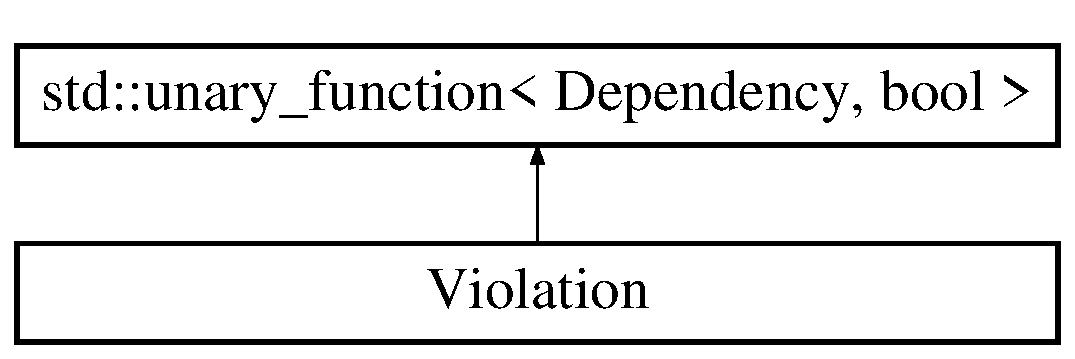
\includegraphics[height=2.000000cm]{struct_violation}
\end{center}
\end{figure}
\subsection*{Public Member Functions}
\begin{DoxyCompactItemize}
\item 
bool \hyperlink{struct_violation_a63407337fcf0ca1a699ee371504533d7}{operator()} (const \hyperlink{class_dependency}{Dependency} \&dep) const 
\end{DoxyCompactItemize}
\subsection*{Friends}
\begin{DoxyCompactItemize}
\item 
class \hyperlink{struct_violation_a7ee004262f27f8c916688911a71e3aa1}{Relation}
\end{DoxyCompactItemize}


\subsection{Detailed Description}
A unary functor class used to test the dependency for the normal form violation. 

The class \hyperlink{struct_violation}{Violation} inherits the unary\+\_\+function to define the unary predicate with \hyperlink{class_dependency}{Dependency} as parameter object. It uses the data members with constant reference to the \hyperlink{class_relation}{Relation} and the constant reference to enumeration value of Noraml to represent the normal form. Note that the it have private constructor to restrict the use of this class limited to only friend class \hyperlink{class_relation}{Relation}. 

\subsection{Member Function Documentation}
\index{Violation@{Violation}!operator()@{operator()}}
\index{operator()@{operator()}!Violation@{Violation}}
\subsubsection[{\texorpdfstring{operator()(const Dependency \&dep) const }{operator()(const Dependency &dep) const }}]{\setlength{\rightskip}{0pt plus 5cm}bool Violation\+::operator() (
\begin{DoxyParamCaption}
\item[{const {\bf Dependency} \&}]{dep}
\end{DoxyParamCaption}
) const\hspace{0.3cm}{\ttfamily [inline]}}\hypertarget{struct_violation_a63407337fcf0ca1a699ee371504533d7}{}\label{struct_violation_a63407337fcf0ca1a699ee371504533d7}
overloaded operator () to be applied as predicate when testing the dependency for the violation. 
\begin{DoxyParams}{Parameters}
{\em dep} & is constant reference to the \hyperlink{class_dependency}{Dependency} object for which the violation is to be tested. \\
\hline
\end{DoxyParams}
\begin{DoxyReturn}{Returns}
true value if it violates the normal form, false otherwise.
\end{DoxyReturn}
The function uses the class member \hyperlink{class_relation}{Relation} and Normal form objects to perform the test against the \hyperlink{class_dependency}{Dependency} object parameter. If the conditions for the particular normal form is violated then the function return true. The different conditions for the normal form violation can be given as follows -\/
\begin{DoxyItemize}
\item Second normal form violation if
\begin{DoxyEnumerate}
\item lhs of \hyperlink{class_dependency}{Dependency} is partial key
\item and rhs is not prime attribute set
\end{DoxyEnumerate}
\item Third normal form violation if
\begin{DoxyEnumerate}
\item lhs of \hyperlink{class_dependency}{Dependency} is not super-\/key
\item and rhs is not prime attribute set
\end{DoxyEnumerate}
\item Boyce-\/\+Codd(BC) normal form violation if
\begin{DoxyEnumerate}
\item lhs of \hyperlink{class_dependency}{Dependency} is not super-\/key 
\end{DoxyEnumerate}
\end{DoxyItemize}

\subsection{Friends And Related Function Documentation}
\index{Violation@{Violation}!Relation@{Relation}}
\index{Relation@{Relation}!Violation@{Violation}}
\subsubsection[{\texorpdfstring{Relation}{Relation}}]{\setlength{\rightskip}{0pt plus 5cm}friend class {\bf Relation}\hspace{0.3cm}{\ttfamily [friend]}}\hypertarget{struct_violation_a7ee004262f27f8c916688911a71e3aa1}{}\label{struct_violation_a7ee004262f27f8c916688911a71e3aa1}
only \hyperlink{class_relation}{Relation} calss have access to construct the object of the \hyperlink{struct_violation}{Violation} struct and to use it. 

The documentation for this struct was generated from the following file\+:\begin{DoxyCompactItemize}
\item 
\hyperlink{violation_8h}{violation.\+h}\end{DoxyCompactItemize}

\chapter{File Documentation}
\hypertarget{declaration_8h}{}\section{declaration.\+h File Reference}
\label{declaration_8h}\index{declaration.\+h@{declaration.\+h}}


Includes declaration of classes and definition of comparator class.  


{\ttfamily \#include \char`\"{}typedef.\+h\char`\"{}}\\*
\subsection*{Classes}
\begin{DoxyCompactItemize}
\item 
class \hyperlink{classsetstr__compare}{setstr\+\_\+compare}
\begin{DoxyCompactList}\small\item\em The function object class for less-\/than inequality comparison of the set of string. \end{DoxyCompactList}\end{DoxyCompactItemize}
\subsection*{Typedefs}
\begin{DoxyCompactItemize}
\item 
typedef set$<$ \hyperlink{typedef_8h_aa234bdb39b1698c1d4955072cfb3195f}{set\+\_\+str}, \hyperlink{classsetstr__compare}{setstr\+\_\+compare} $>$ \hyperlink{declaration_8h_a3205c77c822620c0f6dd4d42ccd70171}{set\+\_\+key}\hypertarget{declaration_8h_a3205c77c822620c0f6dd4d42ccd70171}{}\label{declaration_8h_a3205c77c822620c0f6dd4d42ccd70171}

\begin{DoxyCompactList}\small\item\em A type definition for a set of set of string with set\+\_\+str with the custom compare class \hyperlink{classsetstr__compare}{setstr\+\_\+compare}. \end{DoxyCompactList}\item 
typedef set\+\_\+key\+::iterator \hyperlink{declaration_8h_ad6d8e42b4ed61ab770e0baafba4e84aa}{itr\+\_\+key}\hypertarget{declaration_8h_ad6d8e42b4ed61ab770e0baafba4e84aa}{}\label{declaration_8h_ad6d8e42b4ed61ab770e0baafba4e84aa}

\begin{DoxyCompactList}\small\item\em A type definition for a iterator for set\+\_\+key. \end{DoxyCompactList}\end{DoxyCompactItemize}


\subsection{Detailed Description}
Includes declaration of classes and definition of comparator class. 

This includes the forward declaration of classes from the file \hyperlink{typedef_8h}{typedef.\+h}. It declares the comparator class for set of set of string. It also declares the global type alias for set of the set of string.

\begin{DoxyAuthor}{Author}
Ashish D. Kharde 
\end{DoxyAuthor}

\hypertarget{dependency_8cc}{}\section{dependency.\+cc File Reference}
\label{dependency_8cc}\index{dependency.\+cc@{dependency.\+cc}}


Includes definitions of the \hyperlink{class_dependency}{Dependency} class members defined in the \hyperlink{dependency_8h}{dependency.\+h} file.  


{\ttfamily \#include \char`\"{}dependency.\+h\char`\"{}}\\*
{\ttfamily \#include \char`\"{}utility.\+h\char`\"{}}\\*
{\ttfamily \#include $<$iostream$>$}\\*
{\ttfamily \#include $<$algorithm$>$}\\*


\subsection{Detailed Description}
Includes definitions of the \hyperlink{class_dependency}{Dependency} class members defined in the \hyperlink{dependency_8h}{dependency.\+h} file. 

This file contains definition of the undefined member functions of the class \hyperlink{class_dependency}{Dependency}. 
\hypertarget{dependency_8h}{}\section{dependency.\+h File Reference}
\label{dependency_8h}\index{dependency.\+h@{dependency.\+h}}


Includes declaration for the class \hyperlink{class_dependency}{Dependency} and its members.  


{\ttfamily \#include \char`\"{}declaration.\+h\char`\"{}}\\*
{\ttfamily \#include \char`\"{}utility.\+h\char`\"{}}\\*
{\ttfamily \#include $<$set$>$}\\*
{\ttfamily \#include $<$iostream$>$}\\*
\subsection*{Classes}
\begin{DoxyCompactItemize}
\item 
class \hyperlink{class_dependency}{Dependency}
\begin{DoxyCompactList}\small\item\em The \hyperlink{class_dependency}{Dependency} class that represents the functional dependency of the relation using the attribute set. \end{DoxyCompactList}\end{DoxyCompactItemize}


\subsection{Detailed Description}
Includes declaration for the class \hyperlink{class_dependency}{Dependency} and its members. 

This file declares the definition of the class \hyperlink{class_dependency}{Dependency} along with its subsequent data members and the member functions prototype. 
\hypertarget{relation_8cc}{}\section{relation.\+cc File Reference}
\label{relation_8cc}\index{relation.\+cc@{relation.\+cc}}


Includes definitions of the \hyperlink{class_relation}{Relation} class members defined in the \hyperlink{relation_8h}{relation.\+h} file.  


{\ttfamily \#include \char`\"{}relation.\+h\char`\"{}}\\*
{\ttfamily \#include \char`\"{}utility.\+h\char`\"{}}\\*
{\ttfamily \#include \char`\"{}dependency.\+h\char`\"{}}\\*
{\ttfamily \#include \char`\"{}violation.\+h\char`\"{}}\\*


\subsection{Detailed Description}
Includes definitions of the \hyperlink{class_relation}{Relation} class members defined in the \hyperlink{relation_8h}{relation.\+h} file. 

This file contains definition of all the undefined member functions of the class \hyperlink{class_relation}{Relation}. 
\hypertarget{relation_8h}{}\section{relation.\+h File Reference}
\label{relation_8h}\index{relation.\+h@{relation.\+h}}


Includes declaration for the class \hyperlink{class_relation}{Relation} and its members.  


{\ttfamily \#include \char`\"{}declaration.\+h\char`\"{}}\\*
{\ttfamily \#include \char`\"{}dependency.\+h\char`\"{}}\\*
{\ttfamily \#include $<$set$>$}\\*
{\ttfamily \#include $<$string$>$}\\*
\subsection*{Classes}
\begin{DoxyCompactItemize}
\item 
class \hyperlink{class_relation}{Relation}
\begin{DoxyCompactList}\small\item\em The \hyperlink{class_relation}{Relation} class that represents the relation entity. \end{DoxyCompactList}\end{DoxyCompactItemize}


\subsection{Detailed Description}
Includes declaration for the class \hyperlink{class_relation}{Relation} and its members. 

This file declares the definition of the class \hyperlink{class_relation}{Relation} along with its subsequent data members and the member functions prototype.

\begin{DoxyAuthor}{Author}
Ashish D. Kharde 
\end{DoxyAuthor}

\hypertarget{template__def_8h}{}\section{template\+\_\+def.\+h File Reference}
\label{template__def_8h}\index{template\+\_\+def.\+h@{template\+\_\+def.\+h}}


Contains the definition for various utility template functions.  


{\ttfamily \#include \char`\"{}declaration.\+h\char`\"{}}\\*
{\ttfamily \#include \char`\"{}relation.\+h\char`\"{}}\\*
\subsection*{Functions}
\begin{DoxyCompactItemize}
\item 
{\footnotesize template$<$typename T $>$ }\\bool \hyperlink{template__def_8h_a50aafc8e1ec193cc42a3e6d6d057de8f}{contains} (const set$<$ T $>$ \&list, const T \&val)
\begin{DoxyCompactList}\small\item\em Template function to check whether the second parameter value is present in the set object represented by the first parameter. \end{DoxyCompactList}\item 
{\footnotesize template$<$typename T $>$ }\\bool \hyperlink{template__def_8h_a44b0e719e4225ed6fe6688ec100c0de7}{is\+Equal} (const set$<$ T $>$ \&lhs, const set$<$ T $>$ \&rhs)
\begin{DoxyCompactList}\small\item\em Template function to check the equality of two sets of any datatype. \end{DoxyCompactList}\item 
{\footnotesize template$<$typename T $>$ }\\bool \hyperlink{template__def_8h_ad7698b93a1497654f842e1f3601b2bea}{is\+Subset} (const set$<$ T $>$ \&lhs, const set$<$ T $>$ \&rhs)
\begin{DoxyCompactList}\small\item\em Template function to check whether the second parameter is subset of first of any datatype. \end{DoxyCompactList}\item 
{\footnotesize template$<$typename T $>$ }\\ostream \& \hyperlink{template__def_8h_a6bbaab96bee23ceeacb1a7476f7ac58d}{print\+Set} (ostream \&out, const set$<$ T $>$ \&p\+Set, const \hyperlink{utility_8h_a2b0ed93051b1419873839a5fd176f013}{Parenthesis} \&par)
\begin{DoxyCompactList}\small\item\em Template function to insert the set of any type in the output stream using specified parenthesis. \end{DoxyCompactList}\end{DoxyCompactItemize}


\subsection{Detailed Description}
Contains the definition for various utility template functions. 

Definition of different template method declared in the \hyperlink{utility_8h}{utility.\+h} file. This file is to be included in the \hyperlink{utility_8h}{utility.\+h} file.

\begin{DoxyAuthor}{Author}
Ashish D. Kharde 
\end{DoxyAuthor}


\subsection{Function Documentation}
\index{template\+\_\+def.\+h@{template\+\_\+def.\+h}!contains@{contains}}
\index{contains@{contains}!template\+\_\+def.\+h@{template\+\_\+def.\+h}}
\subsubsection[{\texorpdfstring{contains(const set$<$ T $>$ \&list, const T \&val)}{contains(const set< T > &list, const T &val)}}]{\setlength{\rightskip}{0pt plus 5cm}template$<$typename T $>$ bool contains (
\begin{DoxyParamCaption}
\item[{const set$<$ T $>$ \&}]{list, }
\item[{const T \&}]{val}
\end{DoxyParamCaption}
)\hspace{0.3cm}{\ttfamily [inline]}}\hypertarget{template__def_8h_a50aafc8e1ec193cc42a3e6d6d057de8f}{}\label{template__def_8h_a50aafc8e1ec193cc42a3e6d6d057de8f}


Template function to check whether the second parameter value is present in the set object represented by the first parameter. 


\begin{DoxyParams}{Parameters}
{\em list} & Represents the set of any data-\/type. \\
\hline
{\em val} & Represents the value that need to be search from the parameter set object. \\
\hline
\end{DoxyParams}
\begin{DoxyReturn}{Returns}
true if the val parameter is found in the set parameter list, false otherwise. 
\end{DoxyReturn}
\index{template\+\_\+def.\+h@{template\+\_\+def.\+h}!is\+Equal@{is\+Equal}}
\index{is\+Equal@{is\+Equal}!template\+\_\+def.\+h@{template\+\_\+def.\+h}}
\subsubsection[{\texorpdfstring{is\+Equal(const set$<$ T $>$ \&lhs, const set$<$ T $>$ \&rhs)}{isEqual(const set< T > &lhs, const set< T > &rhs)}}]{\setlength{\rightskip}{0pt plus 5cm}template$<$typename T $>$ bool is\+Equal (
\begin{DoxyParamCaption}
\item[{const set$<$ T $>$ \&}]{lhs, }
\item[{const set$<$ T $>$ \&}]{rhs}
\end{DoxyParamCaption}
)\hspace{0.3cm}{\ttfamily [inline]}}\hypertarget{template__def_8h_a44b0e719e4225ed6fe6688ec100c0de7}{}\label{template__def_8h_a44b0e719e4225ed6fe6688ec100c0de7}


Template function to check the equality of two sets of any datatype. 


\begin{DoxyParams}{Parameters}
{\em lhs} & is the set object that represents first parameter. \\
\hline
{\em rhs} & is the set object that represents second parameter \\
\hline
\end{DoxyParams}
\begin{DoxyReturn}{Returns}
true if both sets are equal, false otherwise.
\end{DoxyReturn}
The function uses the subset method to determine the equality of the two parameter set objects. If lhs is subset of the rhs and rhs is subset of the lhs means both sets are equal. \index{template\+\_\+def.\+h@{template\+\_\+def.\+h}!is\+Subset@{is\+Subset}}
\index{is\+Subset@{is\+Subset}!template\+\_\+def.\+h@{template\+\_\+def.\+h}}
\subsubsection[{\texorpdfstring{is\+Subset(const set$<$ T $>$ \&lhs, const set$<$ T $>$ \&rhs)}{isSubset(const set< T > &lhs, const set< T > &rhs)}}]{\setlength{\rightskip}{0pt plus 5cm}template$<$typename T $>$ bool is\+Subset (
\begin{DoxyParamCaption}
\item[{const set$<$ T $>$ \&}]{lhs, }
\item[{const set$<$ T $>$ \&}]{rhs}
\end{DoxyParamCaption}
)\hspace{0.3cm}{\ttfamily [inline]}}\hypertarget{template__def_8h_ad7698b93a1497654f842e1f3601b2bea}{}\label{template__def_8h_ad7698b93a1497654f842e1f3601b2bea}


Template function to check whether the second parameter is subset of first of any datatype. 


\begin{DoxyParams}{Parameters}
{\em lhs} & is the first parameter represents the set object from which second parameter is to be look up. \\
\hline
{\em rhs} & is the second parameter represents the set object which is to be tested as subset of the first parameter. \\
\hline
\end{DoxyParams}
\begin{DoxyReturn}{Returns}
true if the rhs is subset of the lhs, false otherwise.
\end{DoxyReturn}
The function checks whether every objects from the parameter rhs is present in the parameter lhs. \index{template\+\_\+def.\+h@{template\+\_\+def.\+h}!print\+Set@{print\+Set}}
\index{print\+Set@{print\+Set}!template\+\_\+def.\+h@{template\+\_\+def.\+h}}
\subsubsection[{\texorpdfstring{print\+Set(ostream \&out, const set$<$ T $>$ \&p\+Set, const Parenthesis \&par)}{printSet(ostream &out, const set< T > &pSet, const Parenthesis &par)}}]{\setlength{\rightskip}{0pt plus 5cm}template$<$typename T $>$ ostream\& print\+Set (
\begin{DoxyParamCaption}
\item[{ostream \&}]{out, }
\item[{const set$<$ T $>$ \&}]{p\+Set, }
\item[{const {\bf Parenthesis} \&}]{par}
\end{DoxyParamCaption}
)}\hypertarget{template__def_8h_a6bbaab96bee23ceeacb1a7476f7ac58d}{}\label{template__def_8h_a6bbaab96bee23ceeacb1a7476f7ac58d}


Template function to insert the set of any type in the output stream using specified parenthesis. 


\begin{DoxyParams}{Parameters}
{\em out} & is the output stream object where the set data is to be inserted. \\
\hline
{\em disp\+Set} & is the set objects of any data type T. \\
\hline
{\em par} & is the enumeration object of Parenthesis representing the type of parenthesis to be used when formating the set objects in output stream. Default value is N\+O\+\_\+\+B\+R\+AC in which case no parenthesis will be used to separate set objects. \\
\hline
\end{DoxyParams}
\begin{DoxyReturn}{Returns}
The reference of the out parameter.
\end{DoxyReturn}
This function will insert all the set objects to output stream separated by the parenthesis if necessary. The output operator $<$$<$ should be overloaded for the datatype of the object to insert its content in the output stream. 
\hypertarget{typedef_8h}{}\section{typedef.\+h File Reference}
\label{typedef_8h}\index{typedef.\+h@{typedef.\+h}}


Defines the global type alias for data-\/types.  


{\ttfamily \#include $<$set$>$}\\*
{\ttfamily \#include $<$string$>$}\\*
\subsection*{Typedefs}
\begin{DoxyCompactItemize}
\item 
typedef std\+::string {\bfseries string}\hypertarget{typedef_8h_ad453f9f71ce1f9153fb748d6bb25e454}{}\label{typedef_8h_ad453f9f71ce1f9153fb748d6bb25e454}

\item 
typedef set$<$ \hyperlink{class_relation}{Relation} $>$ \hyperlink{typedef_8h_ae4f64e726e10cd561d68b42cf3a43e94}{set\+\_\+rel}\hypertarget{typedef_8h_ae4f64e726e10cd561d68b42cf3a43e94}{}\label{typedef_8h_ae4f64e726e10cd561d68b42cf3a43e94}

\begin{DoxyCompactList}\small\item\em A type definition for a set of \hyperlink{class_relation}{Relation}. \end{DoxyCompactList}\item 
typedef set$<$ \hyperlink{class_dependency}{Dependency} $>$ \hyperlink{typedef_8h_a49fdcf14d2faf54629fca98482b2dfb9}{set\+\_\+dep}\hypertarget{typedef_8h_a49fdcf14d2faf54629fca98482b2dfb9}{}\label{typedef_8h_a49fdcf14d2faf54629fca98482b2dfb9}

\begin{DoxyCompactList}\small\item\em A type definition for a set of \hyperlink{class_dependency}{Dependency}. \end{DoxyCompactList}\item 
typedef set$<$ string $>$ \hyperlink{typedef_8h_aa234bdb39b1698c1d4955072cfb3195f}{set\+\_\+str}\hypertarget{typedef_8h_aa234bdb39b1698c1d4955072cfb3195f}{}\label{typedef_8h_aa234bdb39b1698c1d4955072cfb3195f}

\begin{DoxyCompactList}\small\item\em A type definition for a set of strings. \end{DoxyCompactList}\item 
typedef set\+\_\+rel\+::iterator \hyperlink{typedef_8h_a0475a58143571a6e2f7a200915ae7359}{itr\+\_\+rel}\hypertarget{typedef_8h_a0475a58143571a6e2f7a200915ae7359}{}\label{typedef_8h_a0475a58143571a6e2f7a200915ae7359}

\begin{DoxyCompactList}\small\item\em A type definition for a iterator of set of \hyperlink{class_relation}{Relation}. \end{DoxyCompactList}\item 
typedef set\+\_\+dep\+::iterator \hyperlink{typedef_8h_ab78cecb3657d8a4377c1f9e4dba8778c}{itr\+\_\+dep}\hypertarget{typedef_8h_ab78cecb3657d8a4377c1f9e4dba8778c}{}\label{typedef_8h_ab78cecb3657d8a4377c1f9e4dba8778c}

\begin{DoxyCompactList}\small\item\em A type definition for a iterator of set of \hyperlink{class_dependency}{Dependency}. \end{DoxyCompactList}\item 
typedef set\+\_\+str\+::iterator \hyperlink{typedef_8h_a2a0262d6db5f9bdfe8d11757ad6c69af}{itr\+\_\+str}\hypertarget{typedef_8h_a2a0262d6db5f9bdfe8d11757ad6c69af}{}\label{typedef_8h_a2a0262d6db5f9bdfe8d11757ad6c69af}

\begin{DoxyCompactList}\small\item\em A type definition for a iterator of set of string. \end{DoxyCompactList}\end{DoxyCompactItemize}
\subsection*{Variables}
\begin{DoxyCompactItemize}
\item 
const unsigned short int \hyperlink{typedef_8h_a48e063c4675a85365eba6fe5ddd90707}{W\+I\+D\+TH} = 12\hypertarget{typedef_8h_a48e063c4675a85365eba6fe5ddd90707}{}\label{typedef_8h_a48e063c4675a85365eba6fe5ddd90707}

\begin{DoxyCompactList}\small\item\em A global constant variable to specify the value of width used in formatting the stream output. \end{DoxyCompactList}\end{DoxyCompactItemize}


\subsection{Detailed Description}
Defines the global type alias for data-\/types. 

Declaration of global type alias and the forward declaration of the classes.

\begin{DoxyAuthor}{Author}
Ashish D. Kharde 
\end{DoxyAuthor}

\hypertarget{user__interface_8cc}{}\section{user\+\_\+interface.\+cc File Reference}
\label{user__interface_8cc}\index{user\+\_\+interface.\+cc@{user\+\_\+interface.\+cc}}


Includes definitions of the \hyperlink{class_user_interface}{User\+Interface} class members defined in the \hyperlink{user__interface_8h}{user\+\_\+interface.\+h} file.  


{\ttfamily \#include \char`\"{}user\+\_\+interface.\+h\char`\"{}}\\*
{\ttfamily \#include $<$iostream$>$}\\*
{\ttfamily \#include $<$regex$>$}\\*
{\ttfamily \#include $<$vector$>$}\\*
{\ttfamily \#include $<$sstream$>$}\\*
{\ttfamily \#include $<$iterator$>$}\\*
{\ttfamily \#include $<$functional$>$}\\*
{\ttfamily \#include $<$algorithm$>$}\\*
{\ttfamily \#include $<$cstdlib$>$}\\*
\subsection*{Macros}
\begin{DoxyCompactItemize}
\item 
\#define \hyperlink{user__interface_8cc_a8b43bafee90b30676faae508c21cb8d7}{P\+R\+I\+NT}~std\+::cout$<$$<$std\+::setw(\hyperlink{typedef_8h_a48e063c4675a85365eba6fe5ddd90707}{W\+I\+D\+TH}) $<$$<$std\+::right$<$$<$ \char`\"{}\char`\"{}
\end{DoxyCompactItemize}
\subsection*{Functions}
\begin{DoxyCompactItemize}
\item 
string {\bfseries get\+Text} (\hyperlink{class_relation_af4a36b464d672235cf91635f0816c95e}{Relation\+::\+Normal} n)\hypertarget{user__interface_8cc_ab2d2a6dd435a19a9881f580902fefb0c}{}\label{user__interface_8cc_ab2d2a6dd435a19a9881f580902fefb0c}

\item 
void {\bfseries print} (std\+::vector$<$ string $>$ \&vec)\hypertarget{user__interface_8cc_a447e8ed30389c2585afa88ef51eda1ce}{}\label{user__interface_8cc_a447e8ed30389c2585afa88ef51eda1ce}

\end{DoxyCompactItemize}


\subsection{Detailed Description}
Includes definitions of the \hyperlink{class_user_interface}{User\+Interface} class members defined in the \hyperlink{user__interface_8h}{user\+\_\+interface.\+h} file. 

This file contains definition of the undefined member functions of the class \hyperlink{class_user_interface}{User\+Interface}. 

\subsection{Macro Definition Documentation}
\index{user\+\_\+interface.\+cc@{user\+\_\+interface.\+cc}!P\+R\+I\+NT@{P\+R\+I\+NT}}
\index{P\+R\+I\+NT@{P\+R\+I\+NT}!user\+\_\+interface.\+cc@{user\+\_\+interface.\+cc}}
\subsubsection[{\texorpdfstring{P\+R\+I\+NT}{PRINT}}]{\setlength{\rightskip}{0pt plus 5cm}\#define P\+R\+I\+NT~std\+::cout$<$$<$std\+::setw({\bf W\+I\+D\+TH}) $<$$<$std\+::right$<$$<$ \char`\"{}\char`\"{}}\hypertarget{user__interface_8cc_a8b43bafee90b30676faae508c21cb8d7}{}\label{user__interface_8cc_a8b43bafee90b30676faae508c21cb8d7}
Defines the global output format using overloaded output with standard ostream object cout. 
\hypertarget{user__interface_8h}{}\section{user\+\_\+interface.\+h File Reference}
\label{user__interface_8h}\index{user\+\_\+interface.\+h@{user\+\_\+interface.\+h}}


Includes declaration for the class \hyperlink{class_user_interface}{User\+Interface} and its members.  


{\ttfamily \#include $<$iomanip$>$}\\*
{\ttfamily \#include $<$vector$>$}\\*
{\ttfamily \#include \char`\"{}declaration.\+h\char`\"{}}\\*
{\ttfamily \#include \char`\"{}relation.\+h\char`\"{}}\\*
\subsection*{Classes}
\begin{DoxyCompactItemize}
\item 
class \hyperlink{class_user_interface}{User\+Interface}
\begin{DoxyCompactList}\small\item\em The \hyperlink{class_user_interface}{User\+Interface} class that represents the interface class which interacts with the user using command line interface and performs the actions accordingly. \end{DoxyCompactList}\end{DoxyCompactItemize}


\subsection{Detailed Description}
Includes declaration for the class \hyperlink{class_user_interface}{User\+Interface} and its members. 

This file declares the definition of the class \hyperlink{class_user_interface}{User\+Interface} along with its subsequent data members and the member functions prototype. 
\hypertarget{utility_8cc}{}\section{utility.\+cc File Reference}
\label{utility_8cc}\index{utility.\+cc@{utility.\+cc}}


Specifies the definitions for the global non-\/member functions defined in \hyperlink{utility_8h}{utility.\+h} header file.  


{\ttfamily \#include \char`\"{}utility.\+h\char`\"{}}\\*
{\ttfamily \#include \char`\"{}dependency.\+h\char`\"{}}\\*
{\ttfamily \#include \char`\"{}relation.\+h\char`\"{}}\\*
{\ttfamily \#include $<$iomanip$>$}\\*
\subsection*{Functions}
\begin{DoxyCompactItemize}
\item 
ostream \& \hyperlink{utility_8cc_ac6f32364e52679f0b1bfcfa0182c29b6}{operator$<$$<$} (ostream \&out, const \hyperlink{declaration_8h_a3205c77c822620c0f6dd4d42ccd70171}{set\+\_\+key} \&disp\+Set)
\begin{DoxyCompactList}\small\item\em Insert set\+\_\+key object into stream. \end{DoxyCompactList}\item 
ostream \& \hyperlink{utility_8cc_a181d1c6ceccf1f145f3cb2006e63d55c}{operator$<$$<$} (ostream \&out, const \hyperlink{typedef_8h_ae4f64e726e10cd561d68b42cf3a43e94}{set\+\_\+rel} \&disp\+Set)\hypertarget{utility_8cc_a181d1c6ceccf1f145f3cb2006e63d55c}{}\label{utility_8cc_a181d1c6ceccf1f145f3cb2006e63d55c}

\begin{DoxyCompactList}\small\item\em Insert set\+\_\+rel objects into stream. \end{DoxyCompactList}\item 
ostream \& \hyperlink{utility_8cc_a8bd018076e968a51710784aaf5df4163}{operator$<$$<$} (ostream \&out, const \hyperlink{typedef_8h_a49fdcf14d2faf54629fca98482b2dfb9}{set\+\_\+dep} \&disp\+Set)\hypertarget{utility_8cc_a8bd018076e968a51710784aaf5df4163}{}\label{utility_8cc_a8bd018076e968a51710784aaf5df4163}

\begin{DoxyCompactList}\small\item\em Insert set\+\_\+dep objects into stream. \end{DoxyCompactList}\item 
ostream \& \hyperlink{utility_8cc_ae1b117ec693ec356470cf1eac7c02dc5}{operator$<$$<$} (ostream \&out, const \hyperlink{typedef_8h_aa234bdb39b1698c1d4955072cfb3195f}{set\+\_\+str} \&disp\+Set)\hypertarget{utility_8cc_ae1b117ec693ec356470cf1eac7c02dc5}{}\label{utility_8cc_ae1b117ec693ec356470cf1eac7c02dc5}

\begin{DoxyCompactList}\small\item\em Insert set\+\_\+str objects into stream. \end{DoxyCompactList}\item 
ostream \& \hyperlink{utility_8cc_a87f00f814efa87ca6c9c1b14f27afdbc}{operator$<$$<$} (ostream \&out, const \hyperlink{class_dependency}{Dependency} \&d)\hypertarget{utility_8cc_a87f00f814efa87ca6c9c1b14f27afdbc}{}\label{utility_8cc_a87f00f814efa87ca6c9c1b14f27afdbc}

\begin{DoxyCompactList}\small\item\em Insert \hyperlink{class_dependency}{Dependency} object into stream. \end{DoxyCompactList}\item 
ostream \& \hyperlink{utility_8cc_a5a0701ff339d703315955ce47b2e2c72}{operator$<$$<$} (ostream \&out, const \hyperlink{class_relation}{Relation} \&rel)\hypertarget{utility_8cc_a5a0701ff339d703315955ce47b2e2c72}{}\label{utility_8cc_a5a0701ff339d703315955ce47b2e2c72}

\begin{DoxyCompactList}\small\item\em Insert \hyperlink{class_relation}{Relation} object into stream. \end{DoxyCompactList}\item 
\hyperlink{declaration_8h_a3205c77c822620c0f6dd4d42ccd70171}{set\+\_\+key} \& \hyperlink{utility_8cc_a00ad2c1b49aca4c16a1b0ec6251c0cfd}{operator-\/=} (\hyperlink{declaration_8h_a3205c77c822620c0f6dd4d42ccd70171}{set\+\_\+key} \&lhs, const \hyperlink{declaration_8h_a3205c77c822620c0f6dd4d42ccd70171}{set\+\_\+key} \&rhs)\hypertarget{utility_8cc_a00ad2c1b49aca4c16a1b0ec6251c0cfd}{}\label{utility_8cc_a00ad2c1b49aca4c16a1b0ec6251c0cfd}

\begin{DoxyCompactList}\small\item\em Subtract and assign the set\+\_\+key objects. \end{DoxyCompactList}\item 
\hyperlink{typedef_8h_aa234bdb39b1698c1d4955072cfb3195f}{set\+\_\+str} \& \hyperlink{utility_8cc_aac4a6fa648409a9d2276bfac8d6fbca5}{operator-\/=} (\hyperlink{typedef_8h_aa234bdb39b1698c1d4955072cfb3195f}{set\+\_\+str} \&lhs, const \hyperlink{typedef_8h_aa234bdb39b1698c1d4955072cfb3195f}{set\+\_\+str} \&rhs)\hypertarget{utility_8cc_aac4a6fa648409a9d2276bfac8d6fbca5}{}\label{utility_8cc_aac4a6fa648409a9d2276bfac8d6fbca5}

\begin{DoxyCompactList}\small\item\em Subtract and assign the set\+\_\+str objects. \end{DoxyCompactList}\item 
bool \hyperlink{utility_8cc_ac4fe94bfc7d70b3abf2cce2859cd8ab6}{test\+Set} (const \hyperlink{declaration_8h_a3205c77c822620c0f6dd4d42ccd70171}{set\+\_\+key} \&lhs, const \hyperlink{typedef_8h_aa234bdb39b1698c1d4955072cfb3195f}{set\+\_\+str} \&rhs, bool super)
\begin{DoxyCompactList}\small\item\em Checks whether the set\+\_\+str object is superset or subset for any set\+\_\+str object of the set\+\_\+key. \end{DoxyCompactList}\end{DoxyCompactItemize}


\subsection{Detailed Description}
Specifies the definitions for the global non-\/member functions defined in \hyperlink{utility_8h}{utility.\+h} header file. 

Definition of the all the non-\/member and non-\/template global functions defined in the header file \hyperlink{utility_8h}{utility.\+h}

\begin{DoxyAuthor}{Author}
Ashish D. Kharde 
\end{DoxyAuthor}


\subsection{Function Documentation}
\index{utility.\+cc@{utility.\+cc}!operator$<$$<$@{operator$<$$<$}}
\index{operator$<$$<$@{operator$<$$<$}!utility.\+cc@{utility.\+cc}}
\subsubsection[{\texorpdfstring{operator$<$$<$(ostream \&out, const set\+\_\+key \&disp\+Set)}{operator<<(ostream &out, const set_key &dispSet)}}]{\setlength{\rightskip}{0pt plus 5cm}ostream\& operator$<$$<$ (
\begin{DoxyParamCaption}
\item[{ostream \&}]{out, }
\item[{const {\bf set\+\_\+key} \&}]{disp\+Set}
\end{DoxyParamCaption}
)}\hypertarget{utility_8cc_ac6f32364e52679f0b1bfcfa0182c29b6}{}\label{utility_8cc_ac6f32364e52679f0b1bfcfa0182c29b6}


Insert set\+\_\+key object into stream. 


\begin{DoxyParams}{Parameters}
{\em ostream} & object where set\+\_\+key objects are inserted. \\
\hline
{\em set\+\_\+key} & object to insert. \\
\hline
\end{DoxyParams}
\begin{DoxyReturn}{Returns}
The same parameter of ostream.
\end{DoxyReturn}
Inserts the all the set\+\_\+str objects from the disp\+Set parameter into the stream with proper formatting, separating each set\+\_\+str objects within the parenthesis and putting all the sets in the curly braces. The empty set\+\_\+key object is indicated by \{ 0 \}. \index{utility.\+cc@{utility.\+cc}!test\+Set@{test\+Set}}
\index{test\+Set@{test\+Set}!utility.\+cc@{utility.\+cc}}
\subsubsection[{\texorpdfstring{test\+Set(const set\+\_\+key \&lhs, const set\+\_\+str \&rhs, bool super)}{testSet(const set_key &lhs, const set_str &rhs, bool super)}}]{\setlength{\rightskip}{0pt plus 5cm}bool test\+Set (
\begin{DoxyParamCaption}
\item[{const {\bf set\+\_\+key} \&}]{lhs, }
\item[{const {\bf set\+\_\+str} \&}]{rhs, }
\item[{bool}]{super}
\end{DoxyParamCaption}
)}\hypertarget{utility_8cc_ac4fe94bfc7d70b3abf2cce2859cd8ab6}{}\label{utility_8cc_ac4fe94bfc7d70b3abf2cce2859cd8ab6}


Checks whether the set\+\_\+str object is superset or subset for any set\+\_\+str object of the set\+\_\+key. 


\begin{DoxyParams}{Parameters}
{\em lhs} & The set\+\_\+key \\
\hline
{\em rhs} & \\
\hline
{\em super} & To determine the type of check either superset true or the subset false. Default value is false for subset. \\
\hline
\end{DoxyParams}
\begin{DoxyReturn}{Returns}
true if the second parameter is subset or superset of the any of first parameter object, false otherwise.
\end{DoxyReturn}
It checks whether the rhs set\+\_\+str object is the super set or the subset of the any of set\+\_\+str object. If it is subset or superset then the it return the true value. The check for either superset or the subset will be determined by the parameter super. 
\hypertarget{utility_8h}{}\section{utility.\+h File Reference}
\label{utility_8h}\index{utility.\+h@{utility.\+h}}


Defines the prototypes for the global non-\/member functions.  


{\ttfamily \#include \char`\"{}declaration.\+h\char`\"{}}\\*
{\ttfamily \#include $<$algorithm$>$}\\*
{\ttfamily \#include $<$iostream$>$}\\*
{\ttfamily \#include $<$set$>$}\\*
{\ttfamily \#include \char`\"{}template\+\_\+def.\+h\char`\"{}}\\*
\subsection*{Enumerations}
\begin{DoxyCompactItemize}
\item 
enum \hyperlink{utility_8h_a2b0ed93051b1419873839a5fd176f013}{Parenthesis} \{ \\*
\hyperlink{utility_8h_a2b0ed93051b1419873839a5fd176f013a9c22339d15445dc6716035fb9d88bf35}{B\+R\+A\+C\+\_\+\+R\+O\+U\+ND}, 
\hyperlink{utility_8h_a2b0ed93051b1419873839a5fd176f013a13b3b5fce47819b5568c8265c92efeb6}{B\+R\+A\+C\+\_\+\+S\+Q\+U\+A\+RE}, 
\hyperlink{utility_8h_a2b0ed93051b1419873839a5fd176f013a3e5200ed8184c6c817b9a5ec5e54e5e8}{B\+R\+A\+C\+\_\+\+C\+U\+R\+LY}, 
\hyperlink{utility_8h_a2b0ed93051b1419873839a5fd176f013a68f6f7993e3967a88a65856e32c16aca}{B\+R\+A\+C\+\_\+\+A\+N\+G\+EL}, 
\\*
\hyperlink{utility_8h_a2b0ed93051b1419873839a5fd176f013ab14b673a4dabf704ca6fc0f623abc5da}{N\+O\+\_\+\+B\+R\+AC}
 \}
\end{DoxyCompactItemize}
\subsection*{Functions}
\begin{DoxyCompactItemize}
\item 
ostream \& \hyperlink{utility_8h_a9fb9b97e81034d3b367ad1efc7bb6347}{operator$<$$<$} (ostream \&, const \hyperlink{class_dependency}{Dependency} \&)\hypertarget{utility_8h_a9fb9b97e81034d3b367ad1efc7bb6347}{}\label{utility_8h_a9fb9b97e81034d3b367ad1efc7bb6347}

\begin{DoxyCompactList}\small\item\em Insert \hyperlink{class_dependency}{Dependency} object into stream. \end{DoxyCompactList}\item 
ostream \& \hyperlink{utility_8h_ae37f6c1025dfc13dc413a73b5b630963}{operator$<$$<$} (ostream \&, const \hyperlink{class_relation}{Relation} \&)\hypertarget{utility_8h_ae37f6c1025dfc13dc413a73b5b630963}{}\label{utility_8h_ae37f6c1025dfc13dc413a73b5b630963}

\begin{DoxyCompactList}\small\item\em Insert \hyperlink{class_relation}{Relation} object into stream. \end{DoxyCompactList}\item 
ostream \& \hyperlink{utility_8h_a02823e2103e10b0b507c5b6dec4c89e2}{operator$<$$<$} (ostream \&, const \hyperlink{declaration_8h_a3205c77c822620c0f6dd4d42ccd70171}{set\+\_\+key} \&)
\begin{DoxyCompactList}\small\item\em Insert set\+\_\+key object into stream. \end{DoxyCompactList}\item 
ostream \& \hyperlink{utility_8h_a7a2a217eb704018e0061c999f219ec9a}{operator$<$$<$} (ostream \&, const \hyperlink{typedef_8h_ae4f64e726e10cd561d68b42cf3a43e94}{set\+\_\+rel} \&)\hypertarget{utility_8h_a7a2a217eb704018e0061c999f219ec9a}{}\label{utility_8h_a7a2a217eb704018e0061c999f219ec9a}

\begin{DoxyCompactList}\small\item\em Insert set\+\_\+rel objects into stream. \end{DoxyCompactList}\item 
ostream \& \hyperlink{utility_8h_a28a31742f70f19aaf08fd911a63b2601}{operator$<$$<$} (ostream \&, const \hyperlink{typedef_8h_aa234bdb39b1698c1d4955072cfb3195f}{set\+\_\+str} \&)\hypertarget{utility_8h_a28a31742f70f19aaf08fd911a63b2601}{}\label{utility_8h_a28a31742f70f19aaf08fd911a63b2601}

\begin{DoxyCompactList}\small\item\em Insert set\+\_\+str objects into stream. \end{DoxyCompactList}\item 
ostream \& \hyperlink{utility_8h_a36db770a902ee60c1e862e53203845ec}{operator$<$$<$} (ostream \&, const \hyperlink{typedef_8h_a49fdcf14d2faf54629fca98482b2dfb9}{set\+\_\+dep} \&)\hypertarget{utility_8h_a36db770a902ee60c1e862e53203845ec}{}\label{utility_8h_a36db770a902ee60c1e862e53203845ec}

\begin{DoxyCompactList}\small\item\em Insert set\+\_\+dep objects into stream. \end{DoxyCompactList}\item 
\hyperlink{declaration_8h_a3205c77c822620c0f6dd4d42ccd70171}{set\+\_\+key} \& \hyperlink{utility_8h_afaed49eb68440594a022212fc851dfa8}{operator-\/=} (\hyperlink{declaration_8h_a3205c77c822620c0f6dd4d42ccd70171}{set\+\_\+key} \&, const \hyperlink{declaration_8h_a3205c77c822620c0f6dd4d42ccd70171}{set\+\_\+key} \&)\hypertarget{utility_8h_afaed49eb68440594a022212fc851dfa8}{}\label{utility_8h_afaed49eb68440594a022212fc851dfa8}

\begin{DoxyCompactList}\small\item\em Subtract and assign the set\+\_\+key objects. \end{DoxyCompactList}\item 
\hyperlink{typedef_8h_aa234bdb39b1698c1d4955072cfb3195f}{set\+\_\+str} \& \hyperlink{utility_8h_a88ae3cd18e95ea0231caa08c8ee2a61c}{operator-\/=} (\hyperlink{typedef_8h_aa234bdb39b1698c1d4955072cfb3195f}{set\+\_\+str} \&, const \hyperlink{typedef_8h_aa234bdb39b1698c1d4955072cfb3195f}{set\+\_\+str} \&)\hypertarget{utility_8h_a88ae3cd18e95ea0231caa08c8ee2a61c}{}\label{utility_8h_a88ae3cd18e95ea0231caa08c8ee2a61c}

\begin{DoxyCompactList}\small\item\em Subtract and assign the set\+\_\+str objects. \end{DoxyCompactList}\item 
bool \hyperlink{utility_8h_a30ecaa2e7bdf98e449b76f60af5c7fa9}{test\+Set} (const \hyperlink{declaration_8h_a3205c77c822620c0f6dd4d42ccd70171}{set\+\_\+key} \&lhs, const \hyperlink{typedef_8h_aa234bdb39b1698c1d4955072cfb3195f}{set\+\_\+str} \&rhs, bool super=false)
\begin{DoxyCompactList}\small\item\em Checks whether the set\+\_\+str object is superset or subset for any set\+\_\+str object of the set\+\_\+key. \end{DoxyCompactList}\item 
string \hyperlink{utility_8h_a6e503c6a8a7a5f732e592b4c649cfcc3}{get\+Brac} (const \hyperlink{utility_8h_a2b0ed93051b1419873839a5fd176f013}{Parenthesis} \&sap, bool close)
\begin{DoxyCompactList}\small\item\em Retrieves the string representing the corresponding parenthesis. \end{DoxyCompactList}\item 
bool \hyperlink{utility_8h_af6edbc383e73073c7271d21b4ab9d982}{contains} (const \hyperlink{declaration_8h_a3205c77c822620c0f6dd4d42ccd70171}{set\+\_\+key} \&list, const \hyperlink{typedef_8h_aa234bdb39b1698c1d4955072cfb3195f}{set\+\_\+str} \&val)
\begin{DoxyCompactList}\small\item\em Checks whether the set\+\_\+str object is present in the set\+\_\+key. \end{DoxyCompactList}\item 
{\footnotesize template$<$typename T $>$ }\\ostream \& \hyperlink{utility_8h_a701a9a4b83f3a1cae26c9da3d0f0ce83}{print\+Set} (ostream \&, const set$<$ T $>$ \&, const \hyperlink{utility_8h_a2b0ed93051b1419873839a5fd176f013}{Parenthesis} \&sap=\hyperlink{utility_8h_a2b0ed93051b1419873839a5fd176f013ab14b673a4dabf704ca6fc0f623abc5da}{N\+O\+\_\+\+B\+R\+AC})
\begin{DoxyCompactList}\small\item\em Template function to insert the set of any type in the output stream using specified parenthesis. \end{DoxyCompactList}\item 
{\footnotesize template$<$typename T $>$ }\\bool \hyperlink{utility_8h_a44b0e719e4225ed6fe6688ec100c0de7}{is\+Equal} (const set$<$ T $>$ \&lhs, const set$<$ T $>$ \&rhs)
\begin{DoxyCompactList}\small\item\em Template function to check the equality of two sets of any datatype. \end{DoxyCompactList}\item 
{\footnotesize template$<$typename T $>$ }\\bool \hyperlink{utility_8h_ad7698b93a1497654f842e1f3601b2bea}{is\+Subset} (const set$<$ T $>$ \&lhs, const set$<$ T $>$ \&rhs)
\begin{DoxyCompactList}\small\item\em Template function to check whether the second parameter is subset of first of any datatype. \end{DoxyCompactList}\item 
{\footnotesize template$<$typename T $>$ }\\bool \hyperlink{utility_8h_a3904e03a9cb58e96a1f374a99122983f}{contains} (const set$<$ T $>$ \&lhs, const T \&val)
\begin{DoxyCompactList}\small\item\em Template function to check whether the second parameter value is present in the set object represented by the first parameter. \end{DoxyCompactList}\end{DoxyCompactItemize}


\subsection{Detailed Description}
Defines the prototypes for the global non-\/member functions. 

Declaration of the prototypes for the global non-\/member functions, overloaded operators and template functions. Also includes the file \hyperlink{template__def_8h}{template\+\_\+def.\+h} which includes the definition of the template functions.

\begin{DoxyAuthor}{Author}
Ashish D. Kharde 
\end{DoxyAuthor}


\subsection{Enumeration Type Documentation}
\index{utility.\+h@{utility.\+h}!Parenthesis@{Parenthesis}}
\index{Parenthesis@{Parenthesis}!utility.\+h@{utility.\+h}}
\subsubsection[{\texorpdfstring{Parenthesis}{Parenthesis}}]{\setlength{\rightskip}{0pt plus 5cm}enum {\bf Parenthesis}}\hypertarget{utility_8h_a2b0ed93051b1419873839a5fd176f013}{}\label{utility_8h_a2b0ed93051b1419873839a5fd176f013}
The global enumerator used for representing the types of the brackets used while producing the output for different sets. \begin{Desc}
\item[Enumerator]\par
\begin{description}
\index{B\+R\+A\+C\+\_\+\+R\+O\+U\+ND@{B\+R\+A\+C\+\_\+\+R\+O\+U\+ND}!utility.\+h@{utility.\+h}}\index{utility.\+h@{utility.\+h}!B\+R\+A\+C\+\_\+\+R\+O\+U\+ND@{B\+R\+A\+C\+\_\+\+R\+O\+U\+ND}}\item[{\em 
B\+R\+A\+C\+\_\+\+R\+O\+U\+ND\hypertarget{utility_8h_a2b0ed93051b1419873839a5fd176f013a9c22339d15445dc6716035fb9d88bf35}{}\label{utility_8h_a2b0ed93051b1419873839a5fd176f013a9c22339d15445dc6716035fb9d88bf35}
}]Represents round brackets \index{B\+R\+A\+C\+\_\+\+S\+Q\+U\+A\+RE@{B\+R\+A\+C\+\_\+\+S\+Q\+U\+A\+RE}!utility.\+h@{utility.\+h}}\index{utility.\+h@{utility.\+h}!B\+R\+A\+C\+\_\+\+S\+Q\+U\+A\+RE@{B\+R\+A\+C\+\_\+\+S\+Q\+U\+A\+RE}}\item[{\em 
B\+R\+A\+C\+\_\+\+S\+Q\+U\+A\+RE\hypertarget{utility_8h_a2b0ed93051b1419873839a5fd176f013a13b3b5fce47819b5568c8265c92efeb6}{}\label{utility_8h_a2b0ed93051b1419873839a5fd176f013a13b3b5fce47819b5568c8265c92efeb6}
}]Represents square/box brackets \index{B\+R\+A\+C\+\_\+\+C\+U\+R\+LY@{B\+R\+A\+C\+\_\+\+C\+U\+R\+LY}!utility.\+h@{utility.\+h}}\index{utility.\+h@{utility.\+h}!B\+R\+A\+C\+\_\+\+C\+U\+R\+LY@{B\+R\+A\+C\+\_\+\+C\+U\+R\+LY}}\item[{\em 
B\+R\+A\+C\+\_\+\+C\+U\+R\+LY\hypertarget{utility_8h_a2b0ed93051b1419873839a5fd176f013a3e5200ed8184c6c817b9a5ec5e54e5e8}{}\label{utility_8h_a2b0ed93051b1419873839a5fd176f013a3e5200ed8184c6c817b9a5ec5e54e5e8}
}]Represents curly brackets \index{B\+R\+A\+C\+\_\+\+A\+N\+G\+EL@{B\+R\+A\+C\+\_\+\+A\+N\+G\+EL}!utility.\+h@{utility.\+h}}\index{utility.\+h@{utility.\+h}!B\+R\+A\+C\+\_\+\+A\+N\+G\+EL@{B\+R\+A\+C\+\_\+\+A\+N\+G\+EL}}\item[{\em 
B\+R\+A\+C\+\_\+\+A\+N\+G\+EL\hypertarget{utility_8h_a2b0ed93051b1419873839a5fd176f013a68f6f7993e3967a88a65856e32c16aca}{}\label{utility_8h_a2b0ed93051b1419873839a5fd176f013a68f6f7993e3967a88a65856e32c16aca}
}]Represents angel brackets \index{N\+O\+\_\+\+B\+R\+AC@{N\+O\+\_\+\+B\+R\+AC}!utility.\+h@{utility.\+h}}\index{utility.\+h@{utility.\+h}!N\+O\+\_\+\+B\+R\+AC@{N\+O\+\_\+\+B\+R\+AC}}\item[{\em 
N\+O\+\_\+\+B\+R\+AC\hypertarget{utility_8h_a2b0ed93051b1419873839a5fd176f013ab14b673a4dabf704ca6fc0f623abc5da}{}\label{utility_8h_a2b0ed93051b1419873839a5fd176f013ab14b673a4dabf704ca6fc0f623abc5da}
}]Represents no brackets \end{description}
\end{Desc}


\subsection{Function Documentation}
\index{utility.\+h@{utility.\+h}!contains@{contains}}
\index{contains@{contains}!utility.\+h@{utility.\+h}}
\subsubsection[{\texorpdfstring{contains(const set\+\_\+key \&list, const set\+\_\+str \&val)}{contains(const set_key &list, const set_str &val)}}]{\setlength{\rightskip}{0pt plus 5cm}bool contains (
\begin{DoxyParamCaption}
\item[{const {\bf set\+\_\+key} \&}]{list, }
\item[{const {\bf set\+\_\+str} \&}]{val}
\end{DoxyParamCaption}
)\hspace{0.3cm}{\ttfamily [inline]}}\hypertarget{utility_8h_af6edbc383e73073c7271d21b4ab9d982}{}\label{utility_8h_af6edbc383e73073c7271d21b4ab9d982}


Checks whether the set\+\_\+str object is present in the set\+\_\+key. 


\begin{DoxyParams}{Parameters}
{\em list} & A constant set of string sets to check from. \\
\hline
{\em val} & A constant string set representing the search value. \\
\hline
\end{DoxyParams}
\begin{DoxyReturn}{Returns}
true for successful find false otherwise.
\end{DoxyReturn}
A alternate version of the template function contains for set of string set with different comparator i.\+e. \hyperlink{classsetstr__compare}{setstr\+\_\+compare}. \index{utility.\+h@{utility.\+h}!contains@{contains}}
\index{contains@{contains}!utility.\+h@{utility.\+h}}
\subsubsection[{\texorpdfstring{contains(const set$<$ T $>$ \&lhs, const T \&val)}{contains(const set< T > &lhs, const T &val)}}]{\setlength{\rightskip}{0pt plus 5cm}template$<$typename T $>$ bool contains (
\begin{DoxyParamCaption}
\item[{const set$<$ T $>$ \&}]{list, }
\item[{const T \&}]{val}
\end{DoxyParamCaption}
)\hspace{0.3cm}{\ttfamily [inline]}}\hypertarget{utility_8h_a3904e03a9cb58e96a1f374a99122983f}{}\label{utility_8h_a3904e03a9cb58e96a1f374a99122983f}


Template function to check whether the second parameter value is present in the set object represented by the first parameter. 


\begin{DoxyParams}{Parameters}
{\em list} & Represents the set of any data-\/type. \\
\hline
{\em val} & Represents the value that need to be search from the parameter set object. \\
\hline
\end{DoxyParams}
\begin{DoxyReturn}{Returns}
true if the val parameter is found in the set parameter list, false otherwise. 
\end{DoxyReturn}
\index{utility.\+h@{utility.\+h}!get\+Brac@{get\+Brac}}
\index{get\+Brac@{get\+Brac}!utility.\+h@{utility.\+h}}
\subsubsection[{\texorpdfstring{get\+Brac(const Parenthesis \&sap, bool close)}{getBrac(const Parenthesis &sap, bool close)}}]{\setlength{\rightskip}{0pt plus 5cm}string get\+Brac (
\begin{DoxyParamCaption}
\item[{const {\bf Parenthesis} \&}]{sap, }
\item[{bool}]{close}
\end{DoxyParamCaption}
)\hspace{0.3cm}{\ttfamily [inline]}}\hypertarget{utility_8h_a6e503c6a8a7a5f732e592b4c649cfcc3}{}\label{utility_8h_a6e503c6a8a7a5f732e592b4c649cfcc3}


Retrieves the string representing the corresponding parenthesis. 


\begin{DoxyParams}{Parameters}
{\em sap} & a constant Parenthesis enumeration object value to represent the type of braces. \\
\hline
{\em close} & a boolean parameter to determine the closing or opening brace. The true value indicates the closing brace and false value indicates the opening brace. \\
\hline
\end{DoxyParams}
\begin{DoxyReturn}{Returns}
The string representing the equivalent value of the parenthesis. The default value will be the empty string. 
\end{DoxyReturn}
\index{utility.\+h@{utility.\+h}!is\+Equal@{is\+Equal}}
\index{is\+Equal@{is\+Equal}!utility.\+h@{utility.\+h}}
\subsubsection[{\texorpdfstring{is\+Equal(const set$<$ T $>$ \&lhs, const set$<$ T $>$ \&rhs)}{isEqual(const set< T > &lhs, const set< T > &rhs)}}]{\setlength{\rightskip}{0pt plus 5cm}template$<$typename T $>$ bool is\+Equal (
\begin{DoxyParamCaption}
\item[{const set$<$ T $>$ \&}]{lhs, }
\item[{const set$<$ T $>$ \&}]{rhs}
\end{DoxyParamCaption}
)\hspace{0.3cm}{\ttfamily [inline]}}\hypertarget{utility_8h_a44b0e719e4225ed6fe6688ec100c0de7}{}\label{utility_8h_a44b0e719e4225ed6fe6688ec100c0de7}


Template function to check the equality of two sets of any datatype. 


\begin{DoxyParams}{Parameters}
{\em lhs} & is the set object that represents first parameter. \\
\hline
{\em rhs} & is the set object that represents second parameter \\
\hline
\end{DoxyParams}
\begin{DoxyReturn}{Returns}
true if both sets are equal, false otherwise.
\end{DoxyReturn}
The function uses the subset method to determine the equality of the two parameter set objects. If lhs is subset of the rhs and rhs is subset of the lhs means both sets are equal. \index{utility.\+h@{utility.\+h}!is\+Subset@{is\+Subset}}
\index{is\+Subset@{is\+Subset}!utility.\+h@{utility.\+h}}
\subsubsection[{\texorpdfstring{is\+Subset(const set$<$ T $>$ \&lhs, const set$<$ T $>$ \&rhs)}{isSubset(const set< T > &lhs, const set< T > &rhs)}}]{\setlength{\rightskip}{0pt plus 5cm}template$<$typename T $>$ bool is\+Subset (
\begin{DoxyParamCaption}
\item[{const set$<$ T $>$ \&}]{lhs, }
\item[{const set$<$ T $>$ \&}]{rhs}
\end{DoxyParamCaption}
)\hspace{0.3cm}{\ttfamily [inline]}}\hypertarget{utility_8h_ad7698b93a1497654f842e1f3601b2bea}{}\label{utility_8h_ad7698b93a1497654f842e1f3601b2bea}


Template function to check whether the second parameter is subset of first of any datatype. 


\begin{DoxyParams}{Parameters}
{\em lhs} & is the first parameter represents the set object from which second parameter is to be look up. \\
\hline
{\em rhs} & is the second parameter represents the set object which is to be tested as subset of the first parameter. \\
\hline
\end{DoxyParams}
\begin{DoxyReturn}{Returns}
true if the rhs is subset of the lhs, false otherwise.
\end{DoxyReturn}
The function checks whether every objects from the parameter rhs is present in the parameter lhs. \index{utility.\+h@{utility.\+h}!operator$<$$<$@{operator$<$$<$}}
\index{operator$<$$<$@{operator$<$$<$}!utility.\+h@{utility.\+h}}
\subsubsection[{\texorpdfstring{operator$<$$<$(ostream \&, const set\+\_\+key \&)}{operator<<(ostream &, const set_key &)}}]{\setlength{\rightskip}{0pt plus 5cm}ostream\& operator$<$$<$ (
\begin{DoxyParamCaption}
\item[{ostream \&}]{out, }
\item[{const {\bf set\+\_\+key} \&}]{disp\+Set}
\end{DoxyParamCaption}
)}\hypertarget{utility_8h_a02823e2103e10b0b507c5b6dec4c89e2}{}\label{utility_8h_a02823e2103e10b0b507c5b6dec4c89e2}


Insert set\+\_\+key object into stream. 


\begin{DoxyParams}{Parameters}
{\em ostream} & object where set\+\_\+key objects are inserted. \\
\hline
{\em set\+\_\+key} & object to insert. \\
\hline
\end{DoxyParams}
\begin{DoxyReturn}{Returns}
The same parameter of ostream.
\end{DoxyReturn}
Inserts the all the set\+\_\+str objects from the disp\+Set parameter into the stream with proper formatting, separating each set\+\_\+str objects within the parenthesis and putting all the sets in the curly braces. The empty set\+\_\+key object is indicated by \{ 0 \}. \index{utility.\+h@{utility.\+h}!print\+Set@{print\+Set}}
\index{print\+Set@{print\+Set}!utility.\+h@{utility.\+h}}
\subsubsection[{\texorpdfstring{print\+Set(ostream \&, const set$<$ T $>$ \&, const Parenthesis \&sap=\+N\+O\+\_\+\+B\+R\+A\+C)}{printSet(ostream &, const set< T > &, const Parenthesis &sap=NO_BRAC)}}]{\setlength{\rightskip}{0pt plus 5cm}template$<$typename T $>$ ostream\& print\+Set (
\begin{DoxyParamCaption}
\item[{ostream \&}]{out, }
\item[{const set$<$ T $>$ \&}]{p\+Set, }
\item[{const {\bf Parenthesis} \&}]{par}
\end{DoxyParamCaption}
)}\hypertarget{utility_8h_a701a9a4b83f3a1cae26c9da3d0f0ce83}{}\label{utility_8h_a701a9a4b83f3a1cae26c9da3d0f0ce83}


Template function to insert the set of any type in the output stream using specified parenthesis. 


\begin{DoxyParams}{Parameters}
{\em out} & is the output stream object where the set data is to be inserted. \\
\hline
{\em disp\+Set} & is the set objects of any data type T. \\
\hline
{\em par} & is the enumeration object of Parenthesis representing the type of parenthesis to be used when formating the set objects in output stream. Default value is N\+O\+\_\+\+B\+R\+AC in which case no parenthesis will be used to separate set objects. \\
\hline
\end{DoxyParams}
\begin{DoxyReturn}{Returns}
The reference of the out parameter.
\end{DoxyReturn}
This function will insert all the set objects to output stream separated by the parenthesis if necessary. The output operator $<$$<$ should be overloaded for the datatype of the object to insert its content in the output stream. \index{utility.\+h@{utility.\+h}!test\+Set@{test\+Set}}
\index{test\+Set@{test\+Set}!utility.\+h@{utility.\+h}}
\subsubsection[{\texorpdfstring{test\+Set(const set\+\_\+key \&lhs, const set\+\_\+str \&rhs, bool super=false)}{testSet(const set_key &lhs, const set_str &rhs, bool super=false)}}]{\setlength{\rightskip}{0pt plus 5cm}bool test\+Set (
\begin{DoxyParamCaption}
\item[{const {\bf set\+\_\+key} \&}]{lhs, }
\item[{const {\bf set\+\_\+str} \&}]{rhs, }
\item[{bool}]{super}
\end{DoxyParamCaption}
)}\hypertarget{utility_8h_a30ecaa2e7bdf98e449b76f60af5c7fa9}{}\label{utility_8h_a30ecaa2e7bdf98e449b76f60af5c7fa9}


Checks whether the set\+\_\+str object is superset or subset for any set\+\_\+str object of the set\+\_\+key. 


\begin{DoxyParams}{Parameters}
{\em lhs} & The set\+\_\+key \\
\hline
{\em rhs} & \\
\hline
{\em super} & To determine the type of check either superset true or the subset false. Default value is false for subset. \\
\hline
\end{DoxyParams}
\begin{DoxyReturn}{Returns}
true if the second parameter is subset or superset of the any of first parameter object, false otherwise.
\end{DoxyReturn}
It checks whether the rhs set\+\_\+str object is the super set or the subset of the any of set\+\_\+str object. If it is subset or superset then the it return the true value. The check for either superset or the subset will be determined by the parameter super. 
\hypertarget{violation_8h}{}\section{violation.\+h File Reference}
\label{violation_8h}\index{violation.\+h@{violation.\+h}}


Includes declaration of functor class \hyperlink{struct_violation}{Violation} used to check violation of any normal form by the \hyperlink{class_dependency}{Dependency} for a \hyperlink{class_relation}{Relation} object.  


{\ttfamily \#include \char`\"{}declaration.\+h\char`\"{}}\\*
{\ttfamily \#include \char`\"{}dependency.\+h\char`\"{}}\\*
{\ttfamily \#include \char`\"{}relation.\+h\char`\"{}}\\*
\subsection*{Classes}
\begin{DoxyCompactItemize}
\item 
struct \hyperlink{struct_violation}{Violation}
\begin{DoxyCompactList}\small\item\em A unary functor class used to test the dependency for the normal form violation. \end{DoxyCompactList}\end{DoxyCompactItemize}


\subsection{Detailed Description}
Includes declaration of functor class \hyperlink{struct_violation}{Violation} used to check violation of any normal form by the \hyperlink{class_dependency}{Dependency} for a \hyperlink{class_relation}{Relation} object. 

This file includes the declaration and definition of class \hyperlink{struct_violation}{Violation} and its subsequent methods.

\begin{DoxyAuthor}{Author}
Ashish D. Kharde 
\end{DoxyAuthor}

%--- End generated contents ---

% Index
\backmatter
\newpage
\phantomsection
\clearemptydoublepage
\addcontentsline{toc}{chapter}{Index}
\printindex

\end{document}
